\documentclass[a4paper,oneside]{book}
\usepackage{meccanica-quantistica}

\hypersetup{
	pdftitle={Meccanica Quantistica},
	pdfauthor={Ferracin Davide},
	pdflang={it},
	pdfsubject={Appunti del corso di Meccanica Quantistica},
	pdfcreator={Davide Ferracin},
	pdfcaptionwriter={Davide Ferracin}
	pdfcopyright={Creative Commons Attribution-ShareAlike 4.0 International},
	pdflicenseurl={http://creativecommons.org/licenses/by-sa/4.0/},
	pdfmetalang={it}
}

% TikZ externalization settings
\usetikzlibrary{external}
\usepgfplotslibrary{external}
\tikzexternalize[prefix=tex/] % output folder

\title{
	{\sffamily\fontsize{35}{42}\selectfont Meccanica Quantistica}
}
\author{
	{\small a cura di}\\
	Davide Ferracin
}
\date{}

\pagestyle{headings}

\addbibresource{meccanica-quantistica.bib}

\begin{document}
\frontmatter
\maketitle

% Colophon
\null % Serve scrivere qualcosa prima di \vfill altrimenti non funziona
\vfill % Riempie lo spazio verticale della pagina
\hspace*{-1.5em}
\includegraphics[scale=.7]{by-sa-icon.pdf}
\begin{flushleft}
	Quest'opera è stata rilasciata con licenza \emph{Creative Commons} Attribuzione - Condividi allo stesso modo 4.0 Internazionale. Per leggere una copia della licenza visita il sito web \url{http://creativecommons.org/licenses/by-sa/4.0/}.\\
	2015, Davide Ferracin (\href{mailto:davide.ferracin@studenti.unimi.it}{\ttfamily davide.ferracin@studenti.unimi.it})\\[1cm]
	Versione aggiornata al \today.
\end{flushleft}

\mainmatter

\chapter{I princ\`ipi della meccanica quantistica}
Vediamo in questo capitolo di porre le fondamenta di questa nuova teoria, inquadrando in una struttura matematica quello che avevamo già visto nell'introduzione, come gli stati, le osservabili e il loro comportamento.
Abbiamo innanzitutto visto la necessità di descrivere gli stati in uno spazio vettoriale, in modo che valga il \emph{principio di sovrapposizione}, e questo stato dovrà essere sul campo complesso per dar luogo a fenomeni di interferenza come nella doppia fenditura.
Lo spazio degli stati, che per ora indichiamo con $\hilbert$, avrà le seguenti proprietà:
\begin{itemize}
	\item è uno spazio vettoriale complesso;
	\item in esso è definito un prodotto scalare definito positivo;
	\item è \emph{completo}, come spazio metrico rispetto alla distanza definita dal prodotto scalare;
	\item è \emph{separabile}, ossia esiste un suo sottoinsieme denso e numerabile;\footnote{Un esempio ``classico'' di spazio separabile è semplicemente $\R$, in cui troviamo $\Q\subset\R$ che è denso e numerabile.} 
\end{itemize}
La completezza implica che tutte le successioni di Cauchy in $\hilbert$ sono anche convergenti, mentre la separabilità assicura l'esistenza di una base ortonormale che abbia cardinalità al più numerabile.
Lo spazio degli stati assuma quindi la struttura di uno \emph{spazio di Hilbert} complesso separabile.

Nella notazione introdotta da Dirac, i vettori di $\hilbert$ sono indicati come \emph{ket}, scritti come $\ket{\cdot}$.
Dobbiamo notare innanzitutto che la corrispondenza tra gli stati fisici e i vettori di questo spazio \emph{non è biunivoca}: mentre un vettore $\ket{x}\in\hilbert$ rappresenta uno e un solo stato fisico, lo stesso stato fisico è rappresentato da $\ket{x}$ e tutti i suoi multipli $\alpha\ket{x}$ per qualsiasi $\alpha\in\C$.
Perciò tutte le informazioni che ricaveremo dal modello quantistico che costruiamo dovranno essere indipendenti da questa arbitrarietà.
Se anzich\'e guardare ai vettori però guardiamo alla classe di vettori che sono tutti multipli (per uno scalare), cioè ai \emph{raggi} dello spazio, allora la corrispondenza diventa s\`i biunivoca.
I ket, quindi, fanno parte di uno spazio vettoriale complesso, dunque ogni combinazione lineare $\alpha\ket{x}+\beta\ket{y}$ è ancora in $\hilbert$.
Il prodotto scalare tra due \emph{ket} è indicato come $\braket{x}{y}$: questa notazione affianca il ket, a destra, con l'elemento a sinistra detto \emph{bra}.
La notazione differente dei due elementi suggerisce una qualche differenza, e in effetti i \emph{ket} e i bra, seppur molto simili, appartengono a due spazi diversi; il prodotto scalare tra due \emph{ket} diventa quindi l'operazione del \emph{bra} associato al primo \emph{ket} sul secondo.
Se i \emph{ket} sono dei vettori di $\hilbert$, possiamo pensare ai \emph{bra} come agli elementi del duale, cioè a funzionali lineari sui ket.
Diamo quindi le proprietà del prodotto scalare cos\`i definito:
\begin{itemize}
	\item è antilineare, ossia $\braket{x}{y}=\braket{y}{x}^*$;
	\item è lineare nella prima variabile, $\braket{x}{\alpha y_1+\beta y_2}=\alpha\braket{x}{y_1}+\beta\braket{x}{y_2}$;
	\item è definito positivo, $\braket{x}{x}\geq 0$ per ogni $\ket{x}\in\hilbert$.
\end{itemize}
Dalle prime due troviamo che è antilineare nella seconda variabile: se vogliamo scomporre il prodotto scalare, dovremo introdurre il coniugato dei componenti, ossia $\braket{\alpha x_1+\beta x_2}{y}=\alpha^*\braket{x_1}{y}+\beta^*\braket{x_2}{y}$.
Dalla terza notiamo infine che il prodotto scalare di un \emph{ket} con se stesso è sempre un numero reale.
Vediamo come costruire questo prodotto scalare: se prendiamo una base ortonormale $\{\ket{e_i}\}$ (quindi $\braket{e_i}{e_j}=\delta_{ij}$), che per semplicità supponiamo finita di cardinalità $n$, allora possiamo esprimere un vettore $\ket{x}$ nei termini di questa base come
\begin{equation}
	\ket{x}=\sum_{i=1}^nx_i\ket{e_i}=x_i\ket{e_i}.
\end{equation}
Analogamente si dà l'espressione di $\ket{y}$, mentre il \emph{bra} associato ad esso è il trasposto coniugato del ket, ossia
\begin{equation}
	\bra{y}=\adj{\ket{y}}=y_i^*\bra{e_i}
\end{equation}
dunque il prodotto scalare tra i due è dato da
\begin{equation}
	\braket{y}{x}=y_j^*x_k\braket{e_j}{e_k}=y_j^*x_k\delta_{jk}=y_j^*x_j,
\end{equation}
che si può anche scrivere come $(y_jx_j^*)^*=\braket{x}{y}^*$, verificando quindi la prima proprietà.

\section{Autovalori e autostati}
Dopo aver inquadrato gli stati del sistema nello spazio di Hilbert con le dovute proprietà, passiamo a studiare le osservabili.
Da un punto di vista prettamente pratico e non matematico possiamo definirle come degli apparecchi che agiscono sul sistema come delle \emph{scatole nere}, di cui non possiamo indagare il funzionamento; successivamente vedremo un modo di definirle anche matematicamente.
Possiamo preoccuparci ora dell'\emph{effetto} che esse producono sul sistema: ad ogni osservabile è associata, chiaramente, una grandezza fisica del sistema, come l'energia, la posizione, eccetera, quindi agendo con un'osservabile sul sistema otteniamo un numero.
Su \emph{come} sia fatto questo numero, però, c'è da discutere.
Sappiamo bene che uno strumento di misura reale ci fornisce una misura con un numero di cifre inevitabilmente finito, quindi questa misura è un numero \emph{razionale}, e il numero di cifre è collegato alla precisione dello strumento.
Possiamo immaginare di aumentare sempre di più questa precisione della misura, ad esempio utilizzando strumenti sempre più sofisticati: nella meccanica classica non si afferma l'esistenza di un limite da porre a questa precisione.
Poich\'e il limite di una successione di numeri razionali è, in generale, un numero reale (dato che $\Q$ non è completo), se aumentiamo indefinitamente la precisione degli strumenti la misura, pur essendo un numero razionale, convergerà ad un numero reale; in effetti la meccanica classica studia i sistemi fisici tramite i numeri reali senza preoccuparsi di questo fatti.

In meccanica quantistica, assumeremo che le osservabili, quindi i nostri strumenti di misura, restituiscano soltanto valori discreti (ma non c'è da preoccuparsi: lo spaziotempo è ancora considerato uno spazio continuo).
Miglioriamo quindi la definizione precedente: diremo che $\xi$ è un'osservabile se è uno ``strumento di misura'' i cui risultati formano un insieme discreto $\{\xi_1,\xi_2,\dots,\xi_n,\dots\}$ (anche infinito).
I valori $\xi_i$ sono detti \emph{autovalori} dell'osservabile $\xi$, e costituiscono quindi i \emph{possibili} risultati della misura.

Torniamo all'esperimento con la lastra polaroid: l'osservabile è la lastra, e il risultato della misura è che il fotone ``passa'' o ``non passa'', e questi due risultati sono quindi gli autovalori.
Associamo al passaggio del fotone l'autovalore 1 e al non passaggio l'autovalore 0.
Non possiamo pretendere di predire il risultato della misura, in generale: sappiamo però che se il fotone è polarizzato linearmente lungo l'asse della lastra, sicuramente passerà, quindi in tale caso avremo con certezza l'autovalore 1.
Analogamente se sappiamo che il fotone è polarizzato ortogonalmente all'asse della lastra, certamente avremo l'autovalore 0.

Più in generale, esistono degli stati del sistema con questa caratteristica: chiamiamo \emph{autostato} un particolare stato del sistema in cui il risultato della misura è certo.
Identificando lo stato con il corrispondente raggio in $\hilbert$, indicheremo con $\ket{\xi_i}$ tale raggio.
Per la corrispondenza biunivoca tra i due elementi, però, spesso chiameremo (impropriamente) stati i raggi di $\hilbert$, per semplificare un poco la notazione.
Dunque indicheremo con $\ket{\xi_i}$ l'autostato dell'osservabile $\xi$ relativo all'autovalore $\xi_i$.
Misurando $\xi$ mentre il sistema è nello stato $\ket{\xi_i}$ siamo certi che otterremo l'autovalore $\xi_i$.
Una volta compiuta la misura, inoltre, abbiamo rimosso ogni incertezza sullo stato attuale del sistema, perch\'e ora lo conosciamo, perciò continuando a misurare la medesima osservabile è chiaro che (almeno negli istanti successivi) otterremo sempre lo stesso risultato: possiamo affermare dunque che se effettuiamo la misura di $\xi$ sul sistema e otteniamo l'autovalore $\xi_i$, allora dopo la misura il sistema si troverà nello stato $\ket{\xi_i}$, che è l'autostato associato all'autovalore.
In generale quindi non ci è dato sapere lo stato del sistema \emph{prima} della misura, ma sapremo in che stato si trova \emph{dopo} averla compiuta: questo è essenzialmente il motivo per cui, compiendo una misura, perturbiamo il sistema.

Prendiamo stavolta due lastre polaroid, allineate lungo lo stesso asse di polarizzazione, e prendiamo gli autovalori 0 e 1 come prima.
Se un fotone passa per le due lastre, è come se misurassimo due volte la sua polarizzazione, quindi rappresentano la stessa osservabile misurata una dopo l'altra.
All'inizio, non sappiamo lo stato del fotone: quando esso passa per la prima lastra, però, può o passare o non passare.
Se passa, cioè se otteniamo 1, il fotone risulta polarizzato lungo l'asse (chiamiamo questo stato $\ket{1}$), quindi certamente passerà anche per la seconda lastra.
Quindi, ricapitolando, misurando il fotone otteniamo 1, dunque siamo sicuri che lo stato del fotone sia $\ket{1}$, che allora passerà anche per la seconda lastra, perch\'e si trova nell'autostato associato all'autovalore 1.
Il discorso è analogo se il fotone non passa attraverso la prima lastra, anche se è una questione un po' delicata perch\'e per la seconda lastra non esiste nemmeno più il fotone da misurare; questo esperimento serve almeno per fissare le idee su questi concetti di base.

Non sempre l'autostato di un autovalore è unico, ma possono esisterne anche di più, anche infiniti: in tal caso, la conoscenza dell'autovalore non determina ancora completamente lo stato del sistema.
Distinguiamo quindi due tipi di osservabili:
\begin{itemize}
	\item quelle \emph{degeneri}, per cui eseguendo la misura non si conosce complessivamente lo stato del sistema (lo è la lastra polaroid: sappiamo la polarizzazione, ma non possiamo conoscere con questo esperiento la frequenza dei fotoni);
	\item quelle \emph{non degeneri}, i cui autovalori determinano completamente lo stato del sistema (corrispondenza biunivoca tra autovalori e stati di $\hilbert$).
\end{itemize}

\section{Probabilità di transizione tra gli stati}
Sappiamo che non possiamo predire il risultato di una misura, a meno che il sistema non sia in un certo autostato: negli altri casi possiamo però sapere la probabilità che un certo risultato si presenti rispetto agli altri.
Il risultato dipenderà quindi sia dallo stato iniziale che da quello di arrivo: cerchiamo ora un metodo per calcolare la probabilità di passare da uno stato $\ket{x}$ allo stato $\ket{y}$.
Questo valore è detto \emph{probabilità di transizione} (dal primo stato all'altro) e lo indicheremo con $P(\ket{x}\to\ket{y})$.
Per determinare questa probabilità usiamo il prodotto scalare: per cominciare, ci serve un numero reale, quindi prendiamo il prodotto scalare $\braket{x}{y}$ per il suo coniugato, ottenendo $P(\ket{x}\to\ket{y})=\abs{\braket{x}{y}}^2$.
Questo però non basta, perch\'e potremmo ottenere un numero maggiore di uno, mentre la probabilità deve essere in $[0,1]$: dobbiamo allora normalizzarla, ottenendo
\begin{equation}
	P(\ket{x}\to\ket{y})=\frac{\abs{\braket{x}{y}}^2}{\braket{x}{x}\braket{y}{y}}.
	\label{eq:probabilita-transizione}
\end{equation}
Possiamo trascurare la normalizzazione se assumiamo tutti gli stati normalizzati: questa assunzione è del tutto legittima, poich\'e sappiamo che se $\ket{x}$ rappresenta un certo stato fisico del sistema allora anche $\alpha\ket{x}$ lo rappresenta per qualsiasi $\alpha\in\C$.
Allora possiamo gli stati $\ket{x}$ e $\frac1{\braket{x}{x}}\ket{x}$ sono equivalenti nella rappresentazione, e il secondo è normalizzato.
Per il momento però consideriamo ancora dei vettori generici, non già normalizzati.
La \eqref{eq:probabilita-transizione} è una buona definizione di probabilità: è certamente positiva, perch\'e $\braket{x}{x}$ e $\braket{y}{y}$ sono positivi (in quanto non sono lo zero di $\hilbert$ e il prodotto scalare non è degenere), e per la disuguaglianza di Schwarz $\abs{\braket{x}{y}}^2\leq\braket{x}{x}\braket{y}{y}$ quindi è anche minore o uguale di 1.
Inoltre essa non dipende dal fattore scalare arbitrario nella corrispondenza tra stati fisici e vettori di $\hilbert$: se al posto di $\ket{x}$ e $\ket{y}$ prendiamo $a\ket{x}$ e $b\ket{y}$ per qualunque $a,b\in\C$, abbiamo
\begin{equation}
	P(a\ket{x}\to b\ket{y})=\frac{\abs{a}^2\abs{b}^2\abs{\braket{x}{y}}^2}{\abs{a}^2\braket{x}{x}\abs{y}^2\braket{y}{y}}=\frac{\abs{\braket{x}{y}}^2}{\braket{x}{x}\braket{y}{y}}=P(\ket{x}\to\ket{y}).
\end{equation}
Infine, questa probabilità è commutativa, cioè $P(\ket{x}\to\ket{y})=P(\ket{y}\to\ket{x})$ come si verifica facilmente scambiando i due ket nella \eqref{eq:probabilita-transizione}.

Prendiamo dunque un'osservabile non degenere $\xi$, e un generico stato $\ket{x}$.
Non sappiamo quale sarà il risultato, ma ogni possibile autovalore $\xi_i$ dell'osservabile avrà una certa probabilità $P_i$ di accadere.
Eseguendo una misura di $\xi$, la probabilità di trovare l'autovalore $\xi_i$ equivale alla probabilità di trovare, dopo la misura, il sistema nell'autostato $\ket{\xi_i}$, quindi è la probabilità di transizione tra $\ket{x}$ e questo autostato:
\begin{equation}
	P_i=\frac{\abs{\braket{\xi_i}{x}}^2}{\braket{\xi_i}{\xi_i}\braket{x}{x}}.
\end{equation}
Ovviamente ogni volta che compiamo la misura dobbiamo ottenere uno degli autovalori, qualunque esso sia, quindi $\sum_kP_k=1$ (gli indici $k$ possono anche essere infiniti).

Se partiamo da un autostato $\ket{\xi_i}$, misurando $\xi$ otterremo sempre con certezza l'autovalore $\xi_i$, quindi la probabilità $P(\ket{\xi_i}\to\ket{\xi_i})$ vale 1.
Come conseguenza abbiamo allora $P(\ket{\xi_i}\to\ket{\xi_k})=0$ per $i\neq k$, dato che la somma di tutte le probabilità è 1, ma allora
\begin{equation}
	P(\ket{\xi_i}\to\ket{\xi_k})=\frac{\abs{\braket{\xi_i}{\xi_k}}^2}{\braket{\xi_i}{\xi_i}\braket{\xi_k}{\xi_k}}=0 \iff \braket{\xi_i}{\xi_k}=0.
	\label{eq:autostati-ortogonali}
\end{equation}
Troviamo allora che
\begin{equation}
	\braket{\xi_i}{\xi_k}=\delta_{ik}
	\label{eq:autostati-ortonormali}
\end{equation}
cioè \emph{due autostati relativi a differenti autovalori sono ortonormali}.

\section{Il postulato di Von Neumann}
Abbiamo dimostrato che gli autostati di un'osservabile non degenere formano un insieme ortonormale.
Esso è anche completo: infatti se esistesse un altro stato $\ket{\phi}$ ortogonale a tutti gli autostati $\ket{\xi_i}$, la probabilità di passare da uno qualunque di questi autostati a $\ket{\phi}$ sarebbe nulla, ma allora $\sum_i\abs{\braket{\xi_i}{\phi}}^2=0$ che è assurdo perch\'e deve essere 1.
Quindi gli autostati (o meglio gli autovettori) di un'osservabile non degenere formano una \emph{base ortonormale} di $\hilbert$.
Chiamiamo \emph{autospazio} relativo all'autovalore $\xi_i$ il sottospazio di $\hilbert$ costituito dagli autostati di tale autovalore.
Se l'osservabile non è degenere, ad ogni autovalore corrisponde un unico autostato, quindi l'autospazio corrispondente ha dimensione 1 (ricordiamo che tutti gli autovettori multipli per uno scalare rappresentano il medesimo stato).
Tutti questi autostati sono anche linearmente indipendenti, in quanto ortonormali, quindi gli autospazi di ciascun autovalore sono tra loro ortogonali (e, ancora, linearmente indipendenti).
Allora detto $\hilbert_i$ l'autospazio dell'autovalore $\xi_i$, possiamo scomporre l'intero spazio $\hilbert$ come somma diretta
\begin{equation}
	\hilbert=\bigoplus_i\hilbert_i.
\end{equation}

Se quindi prendiamo una base di autostati $\{\ket{\xi_i}\}$, possiamo rappresentare ogni stato in termini di questi autostati come
\begin{equation}
	\ket{x}=\sum_ic_i\ket{\xi_i}
\end{equation}
dove i coefficienti $c_i\in\C$ devono soddisfare la condizione $\braket{x}{x}=\sum_ic_i^*c_i=\sum_i\abs{c_i}^2<+\infty$.
Per l'ortonormalità della base possiamo quindi individuare tali coefficienti prendendo il prodotto scalare dello stato $\ket{x}$ con gli autostati, ossia
\begin{equation}
	\braket{\xi_k}{x}=\bra{\xi_k}\sum_ic_i\ket{xi_i}=\sum_ic_i\braket{\xi_k}{\xi_i}=\sum_ic_i\delta_{ik}=c_k,
\end{equation}
ma allora
\begin{equation}
	\ket{x}=\sum_i\braket{\xi_i}{x}\ket{\xi_i}=\sum_i\ket{\xi_i}\braket{\xi_i}{x}=\Big(\sum_i\ket{\xi_i}\bra{\xi_i}\Big)\ket{x}
\end{equation}
da cui ricaviamo che l'operatore $\sum_i\ket{\xi_i}\bra{\xi_i}$ è l'identità su $\hilbert$.
In particolare, il singolo addendo $\ket{\xi_i}\bra{\xi_i}$ è un operatore di \emph{proiezione}, in quanto applicandolo due volte si ha
\begin{equation}
	\ket{\xi_i}\bra{\xi_i}\ket{\xi_i}\bra{\xi_i}=\ket{\xi_i}\braket{\xi_i}{\xi_i}\bra{\xi_i}=\ket{\xi_i}\bra{\xi_i}.
\end{equation}
Inoltre applicandolo ad un vettore si ottiene la sua componente nella direzione di $\ket{\xi_i}$, vale a dire la proiezione di $\ket{x}$ nell'autospazio $\hilbert_i$.
Chiaramente sommando le proiezioni su tutti gli autospazi si ottiene il vettore di partenza, dunque si ha l'operatore identità: questa condizione indica la completezza della base degli autostati.

I discorsi fatti finora valgono solo nel caso di osservabili non degeneri: nell'altro caso, sappiamo che ad un autovalore corrispondono più autostati, che chiaramente dovranno essere linearmente indipendenti (altrimenti rappresenterebbero lo stesso stato fisico).
In questo caso non possiamo sapere in quale autostato si trovi il sistema, ma come al solito possiamo conoscere la probabilità che il sistema si trovi in uno o in un altro.
Per semplicità, consideriamo il caso in cui esistano soltanto di autostati linearmente indipendenti relativi all'autovalore $\xi_1$ di $\xi$: chiamiamo tali autostati $\ket{\xi_1'}$ e $\ket{\xi_1''}$, e assumiamo che gli autovalori $\xi_k$ per $k>1$ non siano degeneri.
Date queste ipotesi allora l'autospazio $\hilbert_1$ ha dimensione 2, ed è chiaramente ortogonale a tutti gli $\hilbert_k$ con $k>1$, quindi anche in questo caso tutti gli $\hilbert_i$ sono linearmente indipendenti e si può scrivere $\hilbert=\bigoplus_i\hilbert_i$.
Possiamo comunque scegliere due vettori linearmente indipendenti da $\hilbert_1$ che insieme agli altri $\ket{\xi_k}$ (sempre $k>1$) formano ancora una base di $\hilbert$; la differenza con le osservabili non degeneri è che ora la base non è più unica, anche a meno di normalizzazioni dei vettori, questo perch\'e in $\hilbert_1$ esistono infinite coppie di vettori linearmente indipendenti anche normalizzati.\footnote{Un caso più ``quotidiano'' analogo a questo lo troviamo nelle basi di $\R$ e di $\R^2$: se consideriamo i vettori a meno di fattori scalari, allora in $\R$ la base può essere una sola (è l'unità) mentre in $\R^2$ ne troviamo infinite, ottenute ruotando la base canonica di un angolo qualsiasi.}

Ad ogni modo, possiamo rappresentare anche in questo caso uno stato $\ket{x}$ in termini della base scelta: abbiamo $\ket{x}=c_1'\ket{\xi_1'}+c_1''\ket{\xi_1''}+\sum_{k>1}c_k\ket{\xi_k}$.
Se abbiamo scelto una base ortonormale, avremo anche in questo caso partendo dallo stato $\ket{x}$ che assumiamo normalizzato, cos\`i come gli autostati, che
\begin{equation}
	\sum_iP_i=\sum_i\abs{\braket{\xi_i}{x}}^2=\sum_i\abs{c_i}^2=\abs{c_1'}^2+\abs{c_1''}^2+\sum_{k>1}\abs{c_k}^2=1,
\end{equation}
dunque per esclusione la probabilità di passare da $\ket{x}$ ad uno stato in $\hilbert_1$ è data da $P_1=1-\sum_{k>1}P_k=1-\sum_{k>1}\abs{c_k}^2=\abs{c_1'}^2+\abs{c_1''}^2$.
Questo discorso è quindi riassunto nel \emph{postulato di Von Neumann}, che afferma
\begin{quote}
	Se una misura di $\xi$ nello stato $\ket{x}$ risulta nell'autovalore $\xi_i$, allora lo stato dopo al misura è dato dalla proiezione di $\ket{x}$ nell'autospazio di $\xi_i$.
\end{quote}
Nel caso precedente tale proiezione è proprio $c_1'\ket{\xi_1'}+c_1''\ket{\xi_1''}$, quindi la probabilità di trovare lo stato nell'autospazio $\hilbert_1$ è $\abs{c_1'}^2+\abs{c_1''}^2$.
Il postulato si può anche riformulare affermando che dopo la misura lo stato del sistema è una combinazione lineare degli autostati relativi all'autovalore trovato: la differenza tra i due enunciati è che nel secondo, per avere gli autostati, dobbiamo specificare una base.
La probabilità di transizione, dunque, non dipende dalla base scelta per $\hilbert$ (come era lecito aspettarsi).

\section{Osservabili e operatori}
Chiamiamo $E_i$ l'operatore dato da $\ket{\xi_i}\bra{\xi_i}$, con $\xi_i$ autovalore di un'osservabile $\xi$ generica.
Per le proprietà viste in precedenza, $E_i^2=E_i$ perch\'e è una proiezione, inoltre ogni stato si può scrivere come $\ket{x}=\sum_i\ket{\xi_i}\braket{\xi_i}{x}=\sum_iE_i\ket{x}$, se scegliamo gli autostati $\ket{\xi_i}$ in modo da avere una base ortonormale.
Assumiamo $\ket{x}$ e gli autostati della base normalizzati: allora se l'osservabile non è degenere la probabilità $P_i$ di trovare l'autovalore $\xi_i$ è la probabilità di transizione da $\ket{x}$ a $\ket{\xi_i}$, data da
\begin{equation}
	P_i=\abs{\braket{x}{\xi_i}}^2=\braket{x}{\xi_i}\braket{x}{\xi_i}^*=\braket{x}{\xi_i}\braket{\xi_i}{x}=\bra{x}E_i\ket{x}.
	\label{eq:probabilita-proiezione-non-degenere}
\end{equation}
Anche nel caso l'osservabile non sia degenere, il risultato non cambia, se prendiamo comunque la proiezione su ogni vettore della base: per linearità, la proiezione di $\ket{x}$ nell'autospazio è la somma delle proiezioni su ciascun vettore della base che appartiene a tale autospazio.
Più praticamente, riprendendo l'autovalore $\xi_1$ visto in precedenza, e assumendo che esso abbia due autovettori linearmente indipendenti $\ket{\xi_1'}$ e $\ket{\xi_1''}$ ortonormali, allora
\begin{equation}
	P_1=\abs{\braket{x}{\xi_1'}}^2+\abs{\braket{x}{\xi_1''}}^2=\bra{x}E_1'\ket{x}+\bra{x}E_1''\ket{x}=\bra{x}(E_1'+E_1'')\ket{x}.
	\label{eq:probabilita-proiezione-degenere}
\end{equation}

Se compiamo un numero $N$ di misure di $\xi$ sullo stato $\ket{x}$ (ovviamente non possiamo farlo consecutivamente: dobbiamo avere $N$ sistemi tutti nello stesso stato e compiere la misura si ciascuno di essi), misureremo ogni autovalore $\xi_i$ un certo numero $n_i$ di volte, con $\sum_in_i=N$.
Possiamo allora definire il valore medio $\avg{\xi}$ dell'osservabile come
\begin{equation}
	\avg{\xi}=\frac1{N}\sum_in_i\xi_i
	\label{eq:valore-medio-finito}
\end{equation}
e per $N\to+\infty$, cioè con un numero infinito di misure, il rapporto $n_i/N$ tende alla probabilità di trovare $\xi_i$, perciò
\begin{equation}
	\avg{\xi}=\sum_iP_i\xi_i
	\label{eq:valore-medio}
\end{equation}
dove le $P_i$ sono definite come al solito finora.
Se il sistema è nello stato $\ket{x}$, dunque, il valore medio è
\begin{equation}
	\avg{\xi}=\sum_i\xi_i\bra{x}E_i\ket{x}=\bra{x}\sum_iE_i\xi_i\ket{x}.
\end{equation}
Definiamo dunque l'\emph{operatore associato} all'osservabile $\xi$ come
\begin{equation}
	\op{\xi}=\sum_i\xi_iE_i.
	\label{eq:definizione-operatore}
\end{equation}
Si ha dunque, se $\ket{x}$ è normalizzato, che $\avg{\xi}=\bra{x}\op{\xi}\ket{x}$, il quale viene infatti chiamato \emph{valore di aspettazione} dell'osservabile $\xi$ sullo stato $\ket{x}$.

Osserviamo subito che gli operatori associati sono hermitiani, ossia $\adj{\op\xi}=\op\xi$: infatti data una base ortonormale di autostati anche degeneri $\{\ket{\xi_i}\}$ si ha
\begin{equation}
	\bra{x}\op{\xi}\ket{y}=\bra{x}\sum_i\xi_iE_i\ket{y}=\sum_i\xi_i\bra{x}E_i\ket{y}=\sum_i\xi_i\braket{x}{\xi_i}\braket{\xi_i}{y},
\end{equation}
e allo stesso tempo
\begin{equation}
	\bra{x}\adj{\op{\xi}}\ket{y}=\bra{y}\op{\xi}\ket{x}^*=\Big(\sum_i\xi_i\braket{y}{\xi_i}\braket{\xi_i}{x}\Big)^*=\sum_i\xi_i\big(\braket{y}{\xi_i}\braket{\xi_i}{x}\big)^*=\sum_i\xi_i\braket{x}{\xi_i}\braket{\xi_i}{y}
\end{equation}
($\sum_i\xi_i\in\R$ quindi è il coniugato di s\'e stesso) che è dunque uguale a $\bra{x}\op{\xi}\ket{y}$.
Inoltre gli autovalori $\xi_i$, che avevamo definito come i possibili risultati della misura dell'osservabile, sono in realtà anche gli autovalori, nel senso matematico, dell'operatore, perch\'e
\begin{equation}
	\op{\xi}\ket{\xi_i}=\sum_k\xi_kE_k\ket{\xi_i}=\sum_k\xi_k\ket{\xi_k}\braket{\xi_k}{\xi_i}=\sum_k\xi_k\ket{\xi_k}\delta_{ik}=\xi_i\ket{\xi_i}.
\end{equation}

Vediamo due importanti proprietà degli operatori hermitiani:
\begin{itemize}
	\item i suoi autovalori sono tutti reali.
		Se infatti $\op\xi\ket{\xi}=\xi\ket{\xi}$, in generale l'autovalore $\xi$ è complesso, ma in questo caso se moltiplichiamo a sinistra per il \emph{bra} $\bra{\xi}$ otteniamo $\bra{\xi}\op\xi\ket{\xi}=\xi\braket{\xi}{\xi}$, ma $\op\xi=\adj{\op\xi}$ quindi $\bra{\xi}\op\xi\ket{\xi}=\bra{\xi}\adj{\op\xi}\ket{\xi}=\bra{\xi}\op\xi\ket{\xi}^*=(\xi\braket{\xi}{\xi})^*$, ossia
		\begin{equation}
			(\xi\braket{\xi}{\xi})^*=\xi\braket{\xi}{\xi}\quad\then\quad\xi^*=\xi
		\end{equation}
		perch\'e $\braket{\xi}{\xi}\in\R$, ma allora $\xi\in\R$.
	\item gli autospazi corrispondenti a differenti autovalori sono ortogonali.
		Prendiamo due autovalori $\eta'$ e $\eta''$ (ovviamente $\eta'\neq\eta''$) dell'operatore $\op\eta$ hermitiano.
		Prendiamo inoltre l'azione di $\op\eta$ su due autostati corrispondenti ai due autovalori, cioè $\op\eta\ket{\eta'}=\eta'\ket{\eta'}$ e $\op\eta=\eta''\ket{\eta''}$.
		Moltiplicando a sinistra per rispettivamente per $\bra{\eta''}$ e $\bra{\eta'}$ otteniamo
		\begin{equation}
			\begin{cases}
				\bra{\eta''}\op\eta\ket{\eta'}=\eta'\braket{\eta''}{\eta'}\\
				\bra{\eta'}\op\eta\ket{\eta''}=\eta''\braket{\eta'}{\eta''}
			\end{cases}
			\quad\then\quad
			\begin{cases}
				\bra{\eta''}\op\eta\ket{\eta'}=\eta'\braket{\eta''}{\eta'}\\
				\bra{\eta''}\op\eta\ket{\eta'}=\eta''^*\braket{\eta''}{\eta'}
			\end{cases}
		\end{equation}
		ma gli autovalori sono reali quindi nella seconda $\eta''^*=\eta''$.
		Allora sottraendo la seconda equazione dalla prima troviamo
		\begin{equation}
			(\eta'-\eta'')\braket{\eta''}{\eta'}=0
		\end{equation}
		ma se $\eta'\neq\eta''$ allora $\braket{\eta''}{\eta'}=0$, ossia i due autostati sono ortogonali.
\end{itemize}

È dunque vero che tutte le osservabili sono operatori hermitiani?
Per quanto visto finora e per come abbiamo associato gli operatori alle osservabili, s\`i, è vero.
Non è vero però il contrario: sappiamo che con gli autostati di un'osservabile, degenere o meno, possiamo costruire una base ortonormale dello spazio degli stati, ma ciò non è sempre possibile con gli operatori hermitiani.
Se lo spazio $\hilbert$ fosse di dimensione finita, allora per il teorema spettrale ogni operatore hermitiano ammette un insieme di autovettori che forma una base dello spazio, ma questo non è più vero in dimensione infinita.
Alcuni operatori infatti, pur essendo hermitiani, non possiedono abbastanza autovettori linearmente indipendenti da poter costruire una base: gli operatori per cui questo accade, invece, si dicono \emph{autoaggiunti}.
Solo quest'ultimo tipo di operatori corrisponde ad un'osservabile; analogamente tutte le osservabili sono operatori autoaggiunti.

\chapter{Rappresentazioni}
Poich\'e i risultati possibili delle misure di osservabili sono gli autovalori dell'operatore associato, è di fondamentale importanza nella meccanica quantistica saper ricavare lo spettro degli operatori.
Gli autovalori più ``importanti'' sono quelli di energia, che formano lo spettro dell'operatore hamiltoniano: dobbiamo quindi risolvere l'\emph{equazione agli autovalori}
\begin{equation}
	\op H\ket{E}=E\ket{E}.
	\label{eq:equazione-autovalori-hamiltoniano}
\end{equation}

Cos\`i come in algebra lineare, per agevolare i calcoli, si è soliti fissare una base e trasformare i vettori di $\R^n$ alle $n$-uple di numeri reali, anche in questo caso conviene passare da una trattazione generica di stati e operatori ad un formalismo più pratico per i calcoli.
Anche in questo caso troviamo degli isomorfismi che trasformano lo spazio degli stati in spazi di Hilberti più comodi: questi isomorfismi sono detti \emph{rappresentazioni}.
Tra le varie rappresentazioni, vedremo quella di Heisenberg e quella di Schr\"odinger.

\section{Rappresentazione di Heisenberg}
Prendiamo un insieme completo ortonormale $\{\ket{i}\}_{i\in\N}$, che forma quindi una base per lo spazio degli stati: possiamo pensare a questa base come al sistema completo di autostati di un'osservabile non degenere.
Abbiamo già visto che si può rappresentare uno stato qualsiasi $\ket{x}$ nei termini di questa base, tramite le proiezioni sui suoi elementi:
\begin{equation}
	\ket{x}=\ser{i}\ket{i}\braket{i}{x}=\ser{i}x_i\ket{i}.
	\label{eq:rappresentazione-stato-heisenberg}
\end{equation}
Il braket $\braket{i}{x}$ fornisce quindi il coefficiente dell'$i$-esimo stato della base.
Il prodotto scalare è dato come, sempre inserendo l'operatore identità,
\begin{equation}
	\braket{x}{y}=\bra{x}\Big(\ser{i}\ket{i}\bra{i}\Big)\ket{y}=\ser{i}\braket{x}{i}\braket{i}{y}=\ser{i}\braket{i}{x}^*\braket{i}{y}=\ser{i}x_i^*y_i
	\label{eq:prodotto-scalare}
\end{equation}
e la norma di uno stato (al quadrato)
\begin{equation}
	\braket{x}{x}=\ser{i}x_i^*x_i=\ser{i}\abs{x_i}^2.
	\label{eq:norma-stato}
\end{equation}
Gli stati $\ket{x}$ e $\ket{y}$ chiaramente esistono e hanno un loro significato indipendentemente dalla base in cui li rappresentiamo.
Con queste associazioni, però, fissata una base possiamo identificare qualsiasi stato tramite i suoi coefficienti $x_i$ che appaiono nella \eqref{eq:rappresentazione-stato-heisenberg}: l'insieme ordinato $\{x_i\}_{i\in\N}$ forma dunque una successione, o un vettore colonna di infinite componenti.
Abbiamo però un ulteriore vincolo, ossia la limitatezza della norma di uno stato: $\braket{x}{x}<+\infty$.
Dunque avremo che
\begin{equation}
	\ser{i}\abs{x_i}^2<+\infty
	\label{eq:successione-quadrato-sommabile}
\end{equation}
ossia la successione $\{x_i\}$ è a \emph{quadrato sommabile}.

Abbiamo trovato dunque un isomorfismo tra lo spazio degli stati e lo spazio delle successioni complesse a quadrato sommabile, che si indica con $\ell^2(\C)$, anch'esso ovviamente uno spazio di Hilbert.
Questo isomorfismo non è canonico, nel senso che è possibile farlo solo tramite la scelta di una base: perciò è sbagliato affermare che la successione $\{x_i\}$ \emph{è} lo stato $\ket{x}$, ma è corretto dire che la successione \emph{rappresenta} lo stato (in una certa base).
Questo isomorfismo è la \emph{rappresentazione di Heisenberg}.

Fissata la rappresentazione degli stati, dobbiamo vedere ora come rappresentare gli operatori: anche qui, l'espressione $\ket{y}=\op A\ket{x}$ non necessita della scelta di una base.
Prendiamo la base $\{\ket{i}\}_{i\in\N}$: per trovare la $i$-esima componente, in questa base, di $\ket{y}$, moltiplichiamo a sinistra i membri per il bra fondamentale $\bra{i}$, ottenendo
\begin{equation}
	\braket{i}{y}=y_i=\bra{i}\op A\ket{x}.
\end{equation}
Introducendo la risoluzione dell'identità tra $\op A$ e $\ket{x}$ troviamo dunque
\begin{equation}
	y_i=\bra{i}\op A\Big(\ser{j}\ket{j}\bra{j}\Big)\ket{x}=\ser{j}\bra{i}\op A\ket{j}\braket{j}{x}=\ser{j}\bra{i}\op A\ket{j}x_j.
	\label{eq:rappresentazione-operatore-matrice}
\end{equation}
Vediamo quindi che l'azione di $\op A$ sullo stato $\ket{x}$ si esprime tramite gli elementi $\bra{i}\op A\ket{j}\defeq A_{ij}$, che sono dei numeri complessi con un doppio indice: chiaramente questi indicano una matrice (di dimensioni infinite). 
L'applicazione dell'operatore $\op A$ allo stato $\ket{x}$ si rappresenta dunque come il prodotto riga per colonna tra la matrice rappresentativa di $\op A$ e il vettore/successione rappresentativo di $\ket{x}$.
Dato un altro operatore $\op B$, il prodotto $\op A\op B$ è rappresentato dalla matrice di componenti $(AB)_{ij}=\bra{i}\op A\op B\ket{j}$, e vediamo che
\begin{equation}
	(AB)_{ij}=\bra{i}\op A\op B\ket{j}=\bra{i}\op A\ser{k}\ket{k}\bra{k}\op B\ket{j}=\ser{k}\bra{i}\op A\ket{k}\bra{k}\op B\ket{j}=\ser{k}A_{ik}B_{kj}
	\label{eq:prodotto-operatori-matrici}
\end{equation}
che è proprio il prodotto riga per colonna delle due matrici rappresentative.
L'aggiunto dell'operatore inoltre è tale che $\bra{i}\adj{\op A}\ket{j}=\bra{j}\op A\ket{i}^*$, cioè $(\adj A)_{ij}=A_{ji}^*$: la matrice rappresentativa dell'aggiunto è la trasposta coniugata di $A$.

Chiarito dunque come si rappresentano stati e operatori, torniamo all'equazione agli autovalori vista all'inizio del capitolo: nella rappresentazione di Heisenberg che abbiamo visto, il metodo più conveniente per risolverla è esprimerla in una base di autostati dell'operatore coinvolto.
Se prendiamo un'osservabile $\xi$ non degenere e i suoi autostati $\{\ket{\xi_i}\}$, che prendiamo normalizzati, abbiamo che
\begin{equation}
	\bra{\xi_i}\op\xi\ket{\xi_j}=\xi_j\braket{\xi_i}{\xi_j}=\xi_j\delta_{ij}
\end{equation}
quindi la matrice rappresentativa è diagonale.

Per la non degenerazione dell'osservabile, ad ogni autovalore corrisponde un solo autovettore, a meno di costanti scalari: questo però non è un problema se ricordiamo che ad uno stato fisico corrisponde un \emph{raggio} nello spazio dei ket, quindi l'autovettore e i suoi multipli rappresentano in realtà lo stesso stato fisico.
La normalizzazione degli autostati già risolve parzialmente questo problema, ma lo stato $\ket{\xi_i}$ e $e^{i\phi_i}\ket{\xi_i}$ rappresentano lo stesso stato fisico e hanno entrambi norma unitaria, di conseguenza c'è ancora una certa arbitrarietà, nella scelta di queste fasi $\phi_i$.
In ogni caso, se al posto di $\ket{\xi_i}$ e $\ket{\xi_j}$ prendiamo gli stati $\ket{\xi_i'}=e^{i\phi_i}\ket{\xi_i}$ e $\ket{\xi_j'}=e^{i\phi_j}\ket{\xi_j}$ troviamo
\begin{equation}
	\braket{\xi_i'}{\xi_j'}=e^{-i\phi_i}\bra{\xi_i}e^{i\phi_j}\ket{\xi_j}=e^{i(\phi_j-\phi_i)}\braket{\xi_i}{\xi_j}=e^{i(\phi_j-\phi_i)}\delta_{ij}
\end{equation}
quindi sono ancora ortonormali: se $i=j$ le fasi si cancellano, mentre se $i\ne j$ si ha $e^{i(\phi_j-\phi_i)}\ne 1$ ma $\delta_{ij}=0$ quindi è comunque nullo.

Se l'osservabile invece è degenere, la scelta di un sistema ortonormale completo di autostati non è più univocamente determinata (a meno di fattori scalari), perch\'e ad ogni autovalore possono corrispondere anche più autostati linearmente indipendenti.
Prendiamo un autovalore degenere $\xi_0$ dell'osservabile $\xi$: se scriviamo la matrice rappresentativa di $\op\xi$ nella base di autostati, l'autospazio $\hilbert_0$ di tale autovalore è lasciato invariato dall'operatore, di conseguenza il blocco di matrice relativo all'autovalore $\xi_0$ è un multiplo dell'identità, e ha dimensione pari al grado di degenerazione dell'autovalore.
La matrice rappresentativa è quindi una matrice a blocchi.
Se prendiamo ora un'osservabile $\eta$ compatibile con $\xi$, le due condividono una base di autostati, perciò possiamo cambiare base in quest'ultima.
In generale, la matrice di $\xi$ anche in questo caso sarà ancora a blocchi: ma lo è anche quella di $\eta$, perch\'e sono compatibili.
Quindi, se $\xi$ è rappresentata da una matrice diagonale, ossia in cui tutti i blocchi hanno dimensione 1, allora anche la matrice di $\eta$ è diagonale.

Aggiungendo altre osservabili compatibili a $\xi$ fino a raggiungere un sistema completo di osservabili, si giunge infine ad una base di autostati ben determinata (senza ``libertà di scelta'' tra autostati linearmente indipendenti in un autospazio) di conseguenza la matrice rappresentativa sarà finalmente diagonale.

\chapter{L'oscillatore armonico}
Il sistema fisico più semplice da studiare in meccanica quantistica, contrariamente alla tradizione, non è la particella libera, in quanto l'operatore impulso (che sarebbe l'unico ad apparire nell'hamiltoniana) è un po' particolare e richiede una trattazione dedicata, che faremo in seguito.
Il sistema più semplice risulta invece essere l'oscillatore armonico, che studiamo qui in una dimensione.
Occupiamoci del problema fondamentale di individuare gli autovalori possibili dell'operatore hamiltoniano, e la loro probabilità associata.
Diamo innanzitutto l'operatore hamiltoniano, in cui sostituiamo già la costante $k$ della forza di richiamo con $m\omega^2$, in modo da evidenziare la frequenza naturale dell'oscillatore ($\omega^2=k/m$):
\begin{equation}
	\op H=\frac1{2m}(\op p^2+m^2\omega^2\op q^2).
	\label{eq:H-oscillatore}
\end{equation}
Chiamiamo $E_0,E_1,\dots,E_n,\dots$ i suoi autovalori, ordinati in modo crescente, ossia con $E_i\leq E_{i+1}$ per ogni $i$, e indichiamo di conseguenza gli autostati corrispondenti con $\ket{E_i}$.
L'autostato $\ket{E_0}$, per cui l'energia è minima, è anche chiamato \emph{autostato fondamentale}.
Cominciamo con un primo importante risultato.
\begin{teorema} \label{t:oscillatore-autovalori-positivi}
	Gli autovalori di $\op H$ di un oscillatore armonico sono tutti positivi.
\end{teorema}
\begin{proof}
	Preso uno stato qualunque $\ket{x}$, il valore di aspettazione dell'energia è
	\begin{equation}
		\avg{H}=\bra{x}\op H\ket{x}=\frac1{2m}(\bra{x}\op p^2\ket{x}+m^2\omega^2\bra{x}\op q^2\ket{x}).
	\end{equation}
	Ora, dato che $\op p$ è hermitiano, $\bra{x}\op p^2\ket{x}=\bra{x}\adj{\op p}\op p\ket{x}$ che è la norma di $\op p\ket{x}$, e lo stesso per la posizione, dunque sono entrambi positivi o nulli: allora $\bra{x}\op H\ket{x}\geq 0$ qualsiasi sia $\ket{x}$.
	Se vale per qualsiasi stato, sarà vero anche per gli autostati $\ket{E_i}$, e se li prendiamo normalizzati allora
	\begin{equation}
		0\leq\bra{E_i}\op H\ket{E_i}=E_i\braket{E_i}{E_i}=E_i
	\end{equation}
	cioè tutti gli autovalori non sono negativi.
	Se prendiamo poi l'autostato fondamentale $\ket{E_0}$, esso non può avere l'autovalore nullo: infatti $E_0=0$ se e solo se $\bra{E_0}\op H\ket{E_0}=0$, vale a dire
	\begin{equation}
		\frac1{2m}(\bra{E_0}\op p^2\ket{E_0}+m^2\omega^2\bra{E_0}\op q\ket{E_0})=0,
	\end{equation}
	ma sono tutti addendi non negativi quindi l'equazione è vera se e solo se $\bra{E_0}\op p^2\ket{E_0}=0$ e contemporaneamente $\bra{E_0}\op q^2\ket{E_0}$.
	Come prima, però, questi due sono la norma di $\op p\ket{E_0}$ e $\op q\ket{E_0}$, e ciò significherebbe che questi due vettori siano nulli, vale a dire $\op q\ket{E_0}=0$ e $\op p\ket{E_0}=0$, e di conseguenza $\ket{E_0}$ sarebbe un autostato simultaneo di $q$ e $p$.
	Questo fatto però viola il rapporto di indeterminazione per cui $\Delta q\Delta p\geq\frac{\hbar}2$ in \emph{qualsiasi} stato: in questo caso invece si avrebbe $\Delta q\Delta p=0$, in quanto sapremmo con precisione posizione e impulso (entrambi nulli).
	Allora è assurdo che $E_0$ sia nullo: se non è nemmeno positivo per quanto dimostrato precedentemente, allora $E_0>0$.
	Dato che $E_0$ è l'autovalore minimo, segue immediatamente che $E_i>0$ per ogni $i$, ossia ogni autovalore di $H$ è positivo.
\end{proof}

Nell'oscillatore armonico riconosciamo anche la simmetria che è presente anche nella controparte classica: i valori di aspettazione della posizione e dell'impulso sono zero, negli autostati di energia.
Infatti, preso un qualunque operatore $\op A$,
\begin{equation}
	\bra{E_i}[\op H,\op A]\ket{E_i}=\bra{E_i}\op H\op A\ket{E_i}-\bra{E_i}\op A\op H\ket{E_i}=E_i^*\bra{E_i}\op p\ket{E_i}-E_i\bra{E_i}\op p\ket{E_i}=0
\end{equation}
in quanto $E_i\in\R$.
Allo stesso tempo, il commutatore con $\op p$ vale
\begin{equation}
	[\op H,\op p]=\frac1{2m}[\op p^2+m^2\omega^2\op q^2,\op p]=\frac1{2m}[\op p^2,\op p]+\frac{m\omega^2}{2}[\op q^2,\op p]=\frac{m\omega^2}2(\op q[\op q,\op p]+[\op q,\op p]\op q)=i\hbar m\omega^2\op q\ne 0
	\label{eq:commutatore-Hp}
\end{equation}
cioè $\op q=[\op H,\op p]/i\hbar m\omega^2$.
Di conseguenza il valore di aspettazione di $q$ da un autostato di energia risulta
\begin{equation}
	\bra{E_i}\op q\ket{E_i}=\frac1{i\hbar m\omega^2}\bra{E_i}[\op H,\op p]\ket{E_i}=0.
\end{equation}
Con lo stesso ragionamento, calcolando $[\op H,\op q]$ si giunge a $\bra{E_i}\op p\ket{E_i}=0$.

Calcoliamo infine lo stato di energia minima: assumendo $\braket{E_0}{E_0}=1$, abbiamo
\begin{equation}
	E_0=\bra{E_0}\op H\ket{E_0}=\frac1{2m}(\bra{E_0}\op p^2\ket{E_0}+m^2\omega^2\bra{E_0}\op q^2\ket{E_0}),
\end{equation}
ma $\bra{E_0}\op p^2\ket{E_0}=\avg{p^2}$, e dato che $\avg{p}=0$ si ha $\Delta p^2=\avg{p^2}-\avg{p}^2=\avg{p^2}$ (analogamente per $q$), quindi\footnote{Sfruttiamo la disuguaglianza $a^2+b^2\ge 2ab$, per $a,b\in\R$: basta considerare $(a-b)^2\ge 0$ per dimostrarla.}
\begin{equation}
	E_0=\frac1{2m}(\avg{p^2}+m^2\omega^2\avg{q^2})=\frac1{2m}(\Delta p^2+m^2\omega^2\Delta q^2)\ge \frac1{2m}2m\omega\Delta p\Delta q=\omega\Delta p\Delta q\ge\frac{\hbar\omega}2,
\end{equation}
e in particolare vale proprio $\hbar\omega/2$ soltanto se $\Delta p=m\omega\Delta q$.
Pertanto lo stato di minima energia, che è allo stesso tempo lo stato di \emph{minima indeterminazione}, è dato da
\begin{equation}
	\begin{cases}
		\Delta p=m\omega\Delta q\\ \Delta p\Delta q=\frac{\hbar}2.
	\end{cases}
	\label{eq:oscillatore-armonico-stato-minima-energia}
\end{equation}

\section{Operatori di creazione e distruzione}
Per calcolare lo spettro dell'hamiltoniano, come faremo nella prossima sezione, ci conviene introdurre due nuovi operatori: definiamo
\begin{equation}
	\op a=\frac1{\sqrt{2\hbar m\omega}}(\op p-im\omega\op q)
	\label{eq:operatore-distruzione}
\end{equation}
e di conseguenza il suo aggiunto
\begin{equation}
	\adj{\op a}=\frac1{\sqrt{2\hbar m\omega}}(\op p+im\omega\op q).
	\label{eq:operatore-creazione}
\end{equation}
Essi sono chiamati rispettivamente operatore di \emph{distruzione} e di \emph{creazione}, per ragioni che vedremo più avanti.
Il loro prodotto è dato da
\begin{multline}
	\adj{\op a}\op a=\frac1{2\hbar m\omega}(\op p+im\omega\op q)(\op p-im\omega\op q)=\frac1{2\hbar m\omega}(\op p^2+im\omega\op q\op p-im\omega\op p\op q+m^2\omega^2\op q^2)=\\=\frac1{2\hbar m\omega}(\op p^2+im\omega[\op q,\op p]+m^2\omega^2\op q^2)=\frac{\op H}{\hbar\omega}+\frac{im\omega[\op q,\op p]}{2\hbar m\omega}=\frac{\op H}{\hbar\omega}-\frac12,
\end{multline}
mentre
\begin{equation}
	\op a\adj{\op a}=\frac{\op H}{\hbar\omega}+\frac12.
\end{equation}
Il commutatore tra i due operatori è dunque $[\op a,\adj{\op a}]=1$.
Possiamo anche ricavare l'hamiltoniano da questi due operatori, trovando che $\op H=\hbar\omega(\adj{\op a}\op a+\frac12)=\hbar\omega(\op a\adj{\op a}-\frac12)$, e di conseguenza
\begin{equation}
	[\op H,\op a]=\hbar\omega[\adj{\op a}\op a, a]=\hbar\omega([\adj{\op a}[\op a,\op a]+[\adj{\op a},\op a]\op a)=-\hbar\omega\op a,
\end{equation}
e anche, dato che il commutatore è antihermitiano, $[\op H,\adj{\op a}]=-\adj{[\op H,\op a]}=\hbar\omega\adj{\op a}$.

Ulteriormente, possiamo definire $\op N=\adj{\op a}\op a$ per ottenere i tre commutatori
\begin{equation}
	[\op a,\adj{\op a}]=1,\qquad [\op N,\op a]=-\op a,\qquad [\op N,\adj{\op a}]=\adj{\op a}.
	\label{eq:algebra-heisenberg}
\end{equation}
L'insieme di questi tre operatori forma un'algebra detta \emph{algebra di Heisenberg}, o algebra del conteggio.

\section{Spettro dell'hamiltoniano}
Sia $\ket{E}$ un autostato di $H$: prendiamo lo stato che risulta applicando l'operatore di distruzione $\op a$ introdotto precedentemente, e questa volta l'azione dell'hamiltoniana è
\begin{equation}
	\op H\op a\ket{E}=(\op H\op a-\op a\op H+\op a\op H)\ket{E}=([\op H,\op a]+\op a\op H)\ket{E}=-\hbar\omega\op a\ket{E}+\op a E\ket{E}=(E-\hbar\omega)\op a\ket{E},
\end{equation}
ossia $\op a\ket{E}$ è ancora un autostato dell'hamiltoniano, ma con l'autovalore (di $H$) diminuito di $\hbar\omega$.
Applicando nuovamente $\op a$ si ottiene un ulteriore autostato con autovalore diminuito di $2\hbar\omega$ rispetto a quello di partenza.
Troviamo quindi una catena di autovalori $\{E,E-\hbar\omega,E-2\hbar\omega,\dots\}$: essa non potrà continuare indefinitamente, perch\'e gli autovalori di $H$ sono tutti positivi.
Infatti si arriverà ad un certo stato $\ket{x}$ tale che $\op a\ket{x}=0$: applicando ancora $\op a$, non troviamo un autovalore diminuito di $\hbar\omega$, ma l'equazione	$\op H\op a\ket{x}=(E-\hbar\omega)\op a\ket{x}$ ma $\op a\ket{x}=0$ quindi essa si riduce a $0=0$, e ci si deve fermare a questo punto della catena di autovalori.
Se $E_0$ è l'autovalore minimo e $\ket{E_0}$ è il suo autostato, esso dovrà avere il valore minimo accettabile di energia, e sarà quindi tale che $\op a\ket{E_0}=0$.
Di conseguenza anche la sua norma è nulla, perciò
\begin{equation}
	0=\bra{E_0}\adj{\op a}\op a\ket{E_0}=\bra{E_0}\frac{\op H}{\hbar\omega}-\frac12\ket{E_0}=\Big(\frac{E_0}{\hbar\omega}-\frac12\Big)\braket{E_0}{E_0}
\end{equation}
poich\'e $\bra{E_0}\op H=\adj{\op H\ket{E_0}}=\op H\ket{E_0}=E_0\ket{E_0}$.
Risulta quindi
\begin{equation}
	E_0=\frac{\hbar\omega}2.
	\label{eq:oscillatore-armonico-energia-minima}
\end{equation}

Se ora guardiamo a $\adj{\op a}$, con un ragionamento analogo troviamo in un autostato di $H$ che
\begin{equation}
	\op H\adj{\op a}\ket{E}=([\op H,\adj{\op a}]+\adj{\op a}\op H)\ket{E}=(E+\hbar\omega)\adj{\op a}\ket{E},
\end{equation}
ossia $\adj{\op a}$ porta ogni autostato dell'hamiltoniano in un altro autostato con autovalore (sempre di $H$) aumentato di $\hbar\omega$.
Dunque, se partiamo da $\ket{E_0}$, possiamo applicare indefinitamente l'operatore o esiste un'energia massima che non si può oltrepassare?
Se esistesse un autostato $\ket{E_M}$ (per il quale $\op H\ket{E_M}=E_M\ket{E_M}$) tale che $\adj{\op a}\ket{E_M}=0$, si avrebbe come prima
\begin{equation}
	0=\bra{E_M}\op a\adj{\op a}\ket{E_M}=\bra{E_M}\frac{\op H}{\hbar\omega}+\frac12\ket{E_M}=\Big(\frac{E_M}{\hbar\omega}+\frac12\Big)\braket{E_M}{E_M},
\end{equation}
ma $E_M=-\hbar\omega/2$ contraddice il fatto che tutti gli autovalori di $H$ sono positivi, quindi un tale autostato non può esistere.

Abbiamo trovato dunque che gli autostati di $H$ soddisfano l'equazione
\begin{equation}
	\op H(\adj{\op a})^k\ket{E_0}=(E_0+k\hbar\omega)(\adj{\op a})^k\ket{E_0}=\Big(\frac{\hbar\omega}2+k\hbar\omega\Big)(\adj{\op a})^k\ket{E_0}=\Big(k+\frac12\Big)\hbar\omega(\adj{\op a})^k\ket{E_0},
\end{equation}
ossia che gli autovalori $E_n$ sono dati da
\begin{equation}
	E_n=\Big(\frac12+n\Big)\hbar\omega
	\label{eq:oscillatore-armonico-autovalori-hamiltoniano}
\end{equation}
per $n\in\{0,1,2,\dots\}$.
Questi devono necessariamente essere tutti e soli gli autovalori perch\'e, se ne esistesse uno con un espressione diversa, applicando $\op a$ ripetutamente non si incontrerebbe più l'autovalore $E_0$ (scendendo a ``gradini'' di $\hbar\omega$, verrebbe saltato) e si scenderebbe cos\`i in autovalori negativi, che è assurdo.
Non conoscendo se $H$ sia degenere o meno, non possiamo però affermare che gli autostati $\ket{E_n}$ relativi a tali autovalori sono unici.\footnote{L'hamiltoniano \emph{non è} degenere, quindi sono realmente tutti e soli gli autostati, ma questo lo dimostreremo più avanti.}

Semplifichiamo dunque la notazione e indichiamo solo con $\ket{n}$ (per $n\in\N_0$) gli autostati dell'hamiltoniano: per quanto visto essi si ottengono tutti applicando ripetutamente $\adj{\op a}$ allo stato fondamentale $\ket{0}$, ma in generale $(\adj{\op a})^n\ket{0}=\ket{n}$ non è normalizzato, anche se lo è $\ket{0}$.
Per calcolare la sua norma, vediamo prima come commutano $\op a$ e $(\adj{\op a})^n$, dato che dobbiamo calcolare $\bra{0}\op a^n(\adj{\op a})^n\ket{0}$.
Abbiamo già visto che $[\op a,\adj{\op a}]=[\op a,(\adj{\op a})^1]=1=1(\adj{\op a})^{1-1}$, dunque potremmo supporre che $[\op a,(\adj{\op a})^n]=n(\adj{\op a})^{n-1}$.
Dimostriamolo per induzione: se assumiamo che $[\op a,(\adj{\op a})^{n-1}]=(n-1)(\adj{\op a})^{n-2}$, allora troviamo
\begin{equation}
	\begin{split}
		[\op a,(\adj{\op a})^n]&=[\op a,\adj{\op a}(\adj{\op a})^{n-1}]=\\
		&=\adj{\op a}[\op a,(\adj{\op a})^{n-1}]+[\op a,\adj{\op a}](\adj{\op a})^{n-1}=\\
		&=\adj{\op a}(n-1)(\adj{\op a})^{n-2}+(\adj{\op a})^{n-1}=\\
		&=(n-1)(\adj{\op a})^{n-1}+(\adj{\op a})^{n-1}=\\
		&=n(\adj{\op a})^{n-1}.
	\end{split}
\end{equation}
Allora, abbiamo
\begin{equation}
	\begin{split}
		\bra{0}\op a^n(\adj{\op a})^n\ket{0}&=\bra{0}\op a^{n-1}\op a(\adj{\op a})^n\ket{0}=\\
		&=\bra{0}\op a^{n-1}\big(\op a(\adj{\op a})^n-(\adj{\op a})^n\op a+(\adj{\op a})^n\op a\big)\ket{0}=\\
		&=\bra{0}\op a^{n-1}[\op a,(\adj{\op a})^n]\ket{0}+\bra{0}\op a^{n-1}(\adj{\op a})^n\op a\ket{0}=\\
		&=\bra{0}\op a^{n-1}[\op a,(\adj{\op a})^n]\ket{0}
	\end{split}
\end{equation}
dove $\bra{0}\op a^{n-1}(\adj{\op a})^n\op a\ket{0}=0$ poich\'e $\op a\ket{0}=0$.
Sostituendo il commutatore con quanto trovato in precedenza, otteniamo
\begin{equation}
	\bra{0}\op a^n(\adj{\op a})^n\ket{0}=n\bra{0}\op a^{n-1}(\adj{\op a})^{n-1}\ket{0},
\end{equation}
di conseguenza iteriamo il calcolo fino ad ottenere
\begin{equation}
	\bra{0}\op a^n(\adj{\op a})^n\ket{0}=n!\braket{0}{0}.
\end{equation}
Per normalizzare gli autostati dell'hamiltoniana li ridefiniamo quindi come
\begin{equation}
	\ket{n}=\frac1{\sqrt{n!}}(\adj{\op a})^n\ket{0},
	\label{eq:oscillatore-armonico-autostati-ortonormali}
\end{equation}
perciò se $\braket{0}{0}=1$ allora anche $\braket{n}{n}=1$ per ogni $n\in\N_0$.


\chapter{Evoluzione temporale}
Poich\'e finora ci siamo interessati degli stati di equilibrio dei sistemi  e delle loro energie, ci è servito studiare soltanto una descrizione indipendente dal tempo.
Per analizzare i fenomeni dinamici e variabili nel tempo, però, ci occorre capire come gli stati dei sistemi quantistici evolvono nel tempo: dato uno stato $\ket{\psi(0)}$ noto ad un certo istante iniziale di tempo, come determinare la sua evoluzione $\ket{\psi(t)}$ ad un generico istante?
Nella meccanica classica questo fenomeno è descritto dall'evoluzione delle coordinate canoniche nello spazio delle fasi; in meccanica quantistica, esso è descritto da un \emph{operatore di propagazione} (o soltanto \emph{propagatore}), sia esso $\op U(t)$, per il quale $\ket{\psi(t)}=\op U(t)\ket{\psi(0)}$.
Seguendo l'esempio della meccanica classica, assumiamo anche qui che l'hamiltoniano sia il generatore delle traslazioni temporali infinitesime.
Se l'hamiltoniano stesso non dipende dal tempo, scriviamo dunque
\begin{equation}
	\op U(t)=e^{-\frac{i}{\hbar}\op Ht}.
	\label{eq:propagatore}
\end{equation}
Notiamo come con questa forma il propagatore rispetta, in modo ovvio, le proprietà che ci aspettiamo possieda:
\begin{itemize}
	\item conserva la probabilità: $\braket{\psi(t)}{\psi(t)}=\bra{\psi(0)}\adj{\op U}(t)\op U(t)\ket{\psi(0)}=\braket{\psi(0)}{\psi(0)}$;
	\item è lineare e continuo, quindi $U(t)\to\op 1$ per $t\to 0$;
	\item si compone con la regola $\op U(t_1)\op U(t_2)=\op U(t_1+t_2)$.
\end{itemize}
In altre parole, qusti operatori formano un gruppo unitario continuo ad un parametro.

Dalla derivata temporale dello stato all'istante $t$, passando alla derivata di $\op U(t)$, possiamo ottenere l'equazione differenziale
\begin{equation}
	\drp{}{t}\ket{\psi(t)}=\drp{}{t}\op U(t)\ket{\psi(0)}=-\frac{i}{\hbar}\op H\op U(t)\ket{\psi(0)}=-\frac{i}{\hbar}\op H\ket{\psi(t)}\quad\longrightarrow\quad \op H=i\hbar\drp{}{t}.
\end{equation}
Nel caso in cui anche l'hamiltoniano dipenda dal tempo, generalizziamo l'equazione nella forma
\begin{equation}
	i\hbar\drp{}{t}\op U(t)=\op H(t)\op U(t)
	\label{eq:schrodinger-tempo}
\end{equation}
detta \emph{equazione di Schr\"odinger dipendente dal tempo}.
Nella rappresentazione delle coordinate troviamo l'equazione differenziale per la funzione d'onda, che è $\bra{q}i\hbar\drp{}{t}\ket{\psi(t)}=\bra{q}\op H(t)\ket{\psi(t)}$ da cui
\begin{equation}
	i\hbar\drp{}{t}\psi(\vec q,t)=H\psi(\vec q,t).
	\label{eq:schrodinger-tempo-coordinate}
\end{equation}

\chapter{Metodi variazionali e di approssimazione}
\section{Il limite classico}
Nella meccanica classica la posizione e l'impulso sono grandezze precise e ben determinate, cosa che sappiamo non accade mai in ambito quantistico.
In alcuni casi potremmi riportarci al primo caso, ad esempio prendendo $\avg{q}$ e $\avg{p}$ alla stregua di variabili classiche se $\Delta q$ e $\Delta p$ sono trascurabili, in quanto i risultati veri mostrerebbero delle fluttuazioni attorno ai valori medi insignificanti.

Ammesso di trovare una situazione ``ideale'', essa può conservarsi nel tempo?
Traduciamo l'equazione di Newton usando i valori medi in $m\ddot{\avg{q}}=\avg{F(q)}$: in linea di principio però $F(\avg{q})\ne\avg{F(q)}$, cosa che accade solo se $F$ è lineare in $q$.
Sviluppando l'espressione della forza centrando in $\avg q$ troviamo $F(q)=F(\avg{q})+(q-\avg{q})F'(\avg{q})+o(q-\avg{q})$ che assume una forma \emph{approssimativamente lineare} quando il resto $o(q-\avg{q})$ è trascurabile.
Tale resto contiene come primo termine, oltretutto, lo scarto quadratico $(q-\avg{q})^2$, che è la quantità da minimizzare per poter compiere l'approssimazione con i valori medi.

Prendiamo il sistema di una particella libera: classicamente abbiamo le equazioni del moto $\dot{p}(t)=0$ e $\dot{q}(t)=\frac{p(t)}m$.
Chiamiamo direttamente $p(t)=p$, che è costante, ottenendo $q(t)=q(0)+\frac{p}{m}t$.
Risulta dunque
\begin{multline}
	\delta q(t)^2=\avg{q^2(t)}-\avg{q(t)}^2=\avg{q^2}+\frac{\avg{p^2}}{m^2}t^2+\frac{t}{m}(\avg{pq}+\avg{qp})-\avg{q}^2-\frac{\avg{p}^2}{m^2}t^2-\frac2{m}\avg{p}\avg{q}t=\\
	=\Delta q(0)^2+\frac{t}{m}(\avg{pq}+\avg{qp}-2\avg{p}\avg{q})+\frac{\Delta p(0)^2}{m^2}t^2
\end{multline}
che è l'equazione di una parabola.
Inesorabilmente quindi avremo $\Delta q(t)\sim\frac{\Delta p}{m}t$ per tempi molto grandi; possiamo concludere che $\Delta q(t)\sim 0$ se la massa della particella è molto grande.

\section{Approssimazione WKB}
Mostriamo il metodo di approssimazione dovuto a Wentzel, Kramers e Brillouin, detto anche \emph{approssimazione semiclassica}.
Consideriamo un sistema di una particella, in una dimensione: se il potenziale è costante, la soluzione dell'equazione di Schr\"odinger è una sovrapposizione di onde piane date da
\begin{equation}
	\psi(x)=\psi(0)e^{\pm ipx/\hbar}
\end{equation}
dove $p=\sqrt{2m(E-V)}$.
Supponiamo ora che $V(x)$, seppur non costante, vari ``lentamente'' in una regione di spazio: qui la funzione d'onda potrebbe essere approssimata proprio come un'onda piana.
Quanto lentamente deve variare il potenziale?
Per trovare la corretta approssimazione pensiamo al fatto che $\hbar$ sia una quantità piccola, trascurabile.
Scriviamo la funzione d'onda nella forma
\begin{equation}
	\psi(x)=e^{i\phi(x)/\hbar}
	\label{eq:WKB-funzione-prova}
\end{equation}
dove $\phi$ è una generica funzione complessa, che sviluppiamo in una serie di potenze di $\hbar$: ogni termine contiene una potenza $\hbar^k$ che moltiplica una certa funzione $\phi_k$, che possiamo vedere come una correzione sempre più fine, all'aumentare di $k$, alla vera funzione d'onda.
Ai nostri fini ci interessano i primi termini: $\phi=\phi_0+\phi_1\hbar+o(\hbar)$.
Prima di tutto calcoliamo le derivate della \eqref{eq:WKB-funzione-prova}: $\psi'=\frac{i}{\hbar}\phi'\psi$ e $\psi''=\frac{i}{\hbar}\phi''\psi-\frac1{\hbar^2}(\phi')^2\psi$.
Riscriviamo l'equazione di Schr\"odinger indipendente dal tempo come
\begin{equation}
	-\frac{\hbar^2}{2m}\psi''+\big[V-E\big]\psi=0\qqq \psi''+\frac{p^2}{\hbar^2}\psi=0
\end{equation}
dove $[p(x)]^2=\frac{2m}{\hbar^2}[E-V(x)]$ e inserendo la \eqref{eq:WKB-funzione-prova} otteniamo
\begin{equation}
	\frac{i}{\hbar}\phi''\psi-\frac1{\hbar^2}(\phi')^2\psi+\frac{p^2}{\hbar^2}\psi=0
\end{equation}
in cui possiamo semplificare $\psi$ in quanto non è mai nulla (è un'esponenziale).
Sostituiamo dunque $\phi$ con il suo sviluppo in serie di potenze di $\hbar$ fino al primo ordine: risulta
\begin{equation}
	\begin{gathered}
		\frac{i}{\hbar}\big[\phi_0''+\phi_1''\hbar+o(\hbar)\big]-\frac1{\hbar^2}\big[\phi_0'+\phi_1'+o(\hbar)\big]^2+\frac{p^2}{\hbar^2}=0\\
		\frac{i}{\hbar}\phi_0''+i\phi_1''+o(1)-\frac1{\hbar^2}\big[(\phi_0')^2+(\phi_1')^2\hbar^2+2\phi_0'\phi_1'\hbar+o(\hbar)\big]+\frac{p^2}{\hbar^2}=0\\
		\frac{i}{\hbar}\phi_0''+i\phi_1''+o(1)-\frac{(\phi_0')^2}{\hbar^2}-(\phi_1')^2-\frac{2\phi_0'\phi_1'}{\hbar}+o\Big(\frac1{\hbar}\Big)=0.
	\end{gathered}
\end{equation}
Moltiplicando tutto per $\hbar^2$ abbiamo
\begin{equation}
	i\hbar\phi_0''+i\hbar^2\phi_1''+o(\hbar^2)-(\phi_0')^2-\hbar^2(\phi_1')^2-2\hbar\phi_0'\phi_1'+p^2+o(\hbar)=0.
\end{equation}
Il termine $o(\hbar^2)$ e tutti gli altri che contengono $\hbar^2$ sono dunque ``assorbiti'' in $o(\hbar)$: abbiamo infine
\begin{equation}
	p^2-(\phi_0')^2+(i\phi_o''-2\phi_0'\phi_1')\hbar+o(\hbar)=0.
	\label{eq:WKB-schroedinger-approssimata}
\end{equation}

Possiamo effettuare dunque un'approssimazione all'ordine zero, cioè considerando solo i termini con la potenza $\hbar^0$ e trascurando i restanti: troviamo $\phi_0'=\abs{p}$, dunque la soluzione dell'equazione di Schr\"odinger con questa approssimazione è
\begin{equation}
	\psi(x)=Ae^{\pm\frac{i}{\hbar}\int p(x')\,\dd x'},
	\label{eq:soluzione-WKB-ordine-0}
\end{equation}
nel senso che una soluzione generale è combinazione lineare delle due onde (una per ciascun segno dell'esponente).
L'integrale è lasciato indefinito in quanto un'eventuale costante arbitraria è assorbita in $A$:
\begin{equation}
	\psi(x)=Ae^{\pm\frac{i}{\hbar}\int p(x')\,\dd x'+c}=Ae^ce^{\pm\frac{i}{\hbar}\int p(x')\,\dd x'}=\tilde{A}e^{\pm\frac{i}{\hbar}\int p(x')\,\dd x'}.
\end{equation}
A questo punto possiamo anche scegliere l'estremo inferiore di integrazione come un generico $x_0$ (nel dominio adatto), trovando
\begin{equation}
	\psi(x)=\psi(0)e^{\pm\frac{i}{\hbar}\int_{x_0}^x p(x')\,\dd x'}.
\end{equation}

Compiamo il passo successivo e consideriamo anche il termine del primo ordine: la funzione d'onda sarà dunque $\psi(x)=A\exp\big(\frac{i}{\hbar}\phi_0(x)+i\phi_1(x)\big)$.
Uguagliando a zero i due termini otteniamo per $\phi_0$ la stessa soluzione trovata poco fa, mentre per il termine in $\hbar$ abbiamo
\begin{equation}
	i\phi_0''=2\phi_0'\phi_1'\qqq \frac{\phi_0''}{\phi_0'}=-2i\phi_1'\qqq \log\phi_0'=-2i\phi_1+k
\end{equation}
per un $k\in\C$ generico.
Risolvendo per $\phi_1$ troviamo, ricordando che $\phi_0'=p$,
\begin{equation}
	\phi_1=\frac{i}2\log\phi_0'+c=i\log\sqrt{\abs{p}}+k'
\end{equation}
perciò la funzione d'onda approssimata è
\begin{equation}
	\psi(x)=Be^{\pm\frac{i}{\hbar}\int^xp(x')\,\dd x'+ik'-\log\sqrt{\abs{p}}}=\frac{B}{\sqrt{p}}e^{\pm\frac{i}{\hbar}\int^xp(x')\,\dd x'},
	\label{eq:soluzione-WKB-ordine-1}
\end{equation}
intendendo anche qui che la soluzione generale è combinazione lineare delle due funzioni, per ciascun segno.

È necessario infine discutere della validità di questa approssimazione: essa è valida se il termine in $\hbar$ è trascurabile, ossia se
\begin{equation}
	\hbar\abs{\drv{}{x}\frac1{p(x)}}\ll 1.
	\label{eq:condizione-approssimazione-WKB}
\end{equation}

\section{Principi variazionali}
Spesso è necessario ricavare i livelli energetici, in particolare quello fondamentale, di un sistema anche quando la soluzione analitica è difficile da trovare.
A questo scopo è utile il metodo variazionale, che ha come punto di partenza la disuguaglianza
\begin{equation}
	E_0\le\frac{\bra{\psi}\op H\ket{\psi}}{\braket{\psi}{\psi}}
	\label{eq:principio-variazionale}
\end{equation}
per ogni stato $\ket{\psi}$ del sistema, dove $E_0$ è l'autovalore minimo dell'hamiltoniano, ossia il livello di energia dello stato fondamentale.
Infatti, espandendo il valore medio $\bra{\psi}\op H\ket{\psi}$ in una base di autostati $\ket{E_n}$ di $\op H$, otteniamo
\begin{equation}
	\bra{\psi}\op H\ket{\psi}=\sum_{n,m}\braket{\psi}{E_n}\bra{E_n}\op H\ket{E_m}\braket{E_m}{\psi}=\sum_{n,m}c_n^*E_m\delta_{nm}c_m=\sum_nE_n\abs{c_n}^2
\end{equation}
dove $c_j=\braket{E_j}{\psi}$.
D'altra parte si ha chiaramente $\braket{\psi}{\psi}=\sum_n\abs{c_n}^2$, perciò
\begin{equation}
	\frac{\bra{\psi}\op H\ket{\psi}}{\braket{\psi}{\psi}}=\frac{\sum_nE_n\abs{c_n}^2}{\sum_n\abs{c_n}^2}\ge\frac{\sum_nE_0\abs{c_n}^2}{\sum_n\abs{c_n}^2}=E_0.
\end{equation}
Possiamo interpretare la frazione come una media pesata degli autovalori $E_n$, dove i pesi sono dati da $\abs{c_n}/\sum_k\abs{c_k}^2$ (sono compresi tra 1 e 0 e la loro somma è 1).

Con questa disuguaglianza potremmo dunque determinare lo stato fondamentale di un sistema, calcolando il valore atteso di $\op H$ per tutti gli stati normalizzati e prendiamo il valore minimo; per ovvi motivi, non è una via perseguibile in pratica.
Ciò che si fa solitamente è considerare, invece che l'intero spazio degli stati possibili, un suo ragionevole sottoinsieme, i cui stati possono essere parametrizzati con delle variabili, in base alle caratteristiche di $\op H$ (in particolare, del potenziale).
Con questa restrizione il valore medio di $\op H$ nella \eqref{eq:principio-variazionale} diventa una funzione di queste variabili scelte, di cui possiamo comodamente calcolare il minimo, che è quindi una maggiorazione di $E_0$.
Ad esempio, se il potenziale è pari e vogliamo cercare lo stato fondamentale, proveremo uno stato caratterizzato da una funzione d'onda pari, senza nodi e che ovviamente sia a quadrato sommabile.
Una volta trovato un valore però non possiamo sapere, senza altre informazioni, se è una buona stima di $E_0$; potremmo addirittura trovare il valore esatto di $E_0$.
La bontà della stima è data innanzitutto da come modelliamo lo ``stato prova'' su cui calcoliamo $\bra{\psi}\op H\ket{\psi}$: ad esempio uno stato con funzione d'onda dispari e qualche nodo non darà certamente buoni risultati per lo stato fondamentale.
Possiamo ad esempio riprovare la stima questa volta aggiungendo altri parametri allo stato, cercando di trovare una stima di $E_0$ minore della precedente.
Più elaborato è il modello di prova, migliore sarà l'approssimazione: d'altro canto, continuando ad aggiungere parametri la mole di calcoli da compiere aumenta sempre di più, e potrebbe non valerne la pena se i miglioramenti su $E_0$ non sono apprezzabili.
Lo scopo di questo metodo è, in un certo senso, trovare la migliore approssimazione con il minor lavoro possibile.


\chapter{Sistemi unidimensionali}
In queto capitolo affronteremo una serie di esempi ``accademici'' di sistemi in una dimensione, cercando di risolvere dove possibile l'equazione di Schr\"odinger per la funzione d'onda e lo spettro di energia, o di trovare la migliore approssimazione sfruttando le tecniche acquisite.

\chapter{Momento angolare}
L'operatore associato al momento angolare è, come in meccanica classica, il generatore delle rotazioni, che soddisfa le relazioni di commutazione
\begin{equation}
	[\op L_i,\op L_j]=i\hbar\epsilon_{ijk}\op L_k.
	\label{eq:commutazione-momento-angolare}
\end{equation}
A meno di fattori moltiplicativi, le costanti di struttura (la parte rilevante è il simbolo di Levi-Civita $\epsilon_{ijk}$) sono le stesse dell'algebra di Lie $\mathfrak{su}(2)$.
Non a caso, $\mathfrak{su}(2)$ è isomorfa a $\mathfrak{so}(3)$ che è l'algebra del gruppo $SO(3)$ delle rotazioni tridimensionali; in altre parole $\mathfrak{su}(2)$ genera $SO(3)$, allo stesso modo in cui il momento angolare genera le rotazioni in $\R^3$, e ciò giustifica la \eqref{eq:commutazione-momento-angolare}.
Una quantità che commuta con il momento angolare lungo una data direzione è dunque simmetrica per le rotazioni attorno a tale asse: gli scalari sono degli importanti esempi di queste quantità.
\footnote{
	Spesso si usa, per alleggerire la notazione, porre $\hbar=1$ per eliminarlo sistematicamente dalle equazioni.
	In tal caso si suppone di misurare il momento angolare (e le osservabili che ne derivano) in unità di $\hbar$.
	In pratica, il punto di partenza è dividere la \eqref{eq:commutazione-momento-angolare} per $\hbar^2$ ottenendo la forma più semplice $[\op L_i,\op L_j]=i\epsilon_{ijk}\op L_k$.
}
Insieme alle tre componenti cartesiane del momento angolare abbiamo anche il quadrato del suo modulo, ossia $\op{\vec L}^2=\op L_i\op L_i$: essendo uno scalare, ci aspettiamo che sia invariante per rotazioni ossia che commuti con tutte le componenti del momento angolare.
Una verifica diretta mostra infatti che, per $i=1,2,3$,
\begin{equation}
	[\op{\vec L}^2,\op L_i]=[\op L_k\op L_k,\op L_i]=\op L_k[\op L_k,\op L_i]+[\op L_k,\op L_i]\op L_k=i\hbar\epsilon_{kil}(\op L_k\op L_l+\op L_l\op L_k)=i\hbar(\epsilon_{kil}+\epsilon_{lik})\op L_k\op L_l=0
\end{equation}
per l'antisimmetria di $\epsilon_{kil}$.
In ogni caso le tre componenti $\op L_i$ non sono tra loro compatibili (dalla \eqref{eq:commutazione-momento-angolare}) a meno del caso banale in cui siano tutte nulle.
Nella costruzione di un sistema completo di osservabili compatibili, è convenzione scegliere insieme a $\op{\vec L}^2$ anche la componente $z$, ossia $\op L_3$, da diagonalizzare simultaneamente.

\section{Autovalori del momento angolare} \label{sec:autovalori-momento-angolare}
Supponiamo di aver trovato un sistema completo di osservabili compatibili che contenga $\op{\vec L}^2$ e $\op L^3$.
Chiamiamo $m\hbar$ gli autovalori di $\op L_3$ e $\mu^2\hbar^2$ quelli di $\op{\vec L}^2$, e trascurando lo altre osservabili del sistema indichiamo gli autostati simultanei con $\ket{m,\mu^2}$, che sono quindi tali per cui\footnote{Gli autovalori di $\op{\vec L}^2$ sono evidentemente positivi, perciò li indichiamo direttamente con il quadrato $\mu^2$.}
\begin{equation}
	\op{\vec L}^2\ket{m,\mu^2}=\mu^2\hbar^2\ket{m,\mu^2}
	\hspace{1cm}\text{e}\hspace{1cm}
	\op L_3\ket{m,\mu^2}=m\hbar\ket{m,\mu^2}.
\end{equation}
Come già per l'oscillatore armonico, introduciamo gli operatori a scala $\op L_+\defeq\op L_1+i\op L_2$ e $\op L_-\defeq\op L_1-i\op L_2$.
Dato che gli $\op L_i$ sono hermitiani (poich\'e rappresentano delle osservabili) si vede subito che $\adj{\op L_+}=\op L_-$.
Essi sono in relazione con la componente scelta del momento angolare con i commutatori
\begin{equation}
	[\op L_3,\op L_+]=[\op L_3,\op L_1]+i[\op L_3,\op L_2]=\hbar(i\op L_2-i^2\op L_1)=\hbar\op L_+
\end{equation}
da cui
\begin{equation}
	[\op L_3,\op L_-]=[\op L_3,\adj{\op L_+}]=-\adj{[\op L_3,\op L_+]}=-\hbar\adj{\op L_+}=-\hbar\op L_-.
\end{equation}
Vediamo dunque come questi due operatori agiscono sugli autostati:
\begin{multline}
	\op L_3\op L_+\ket{m,\mu^2}=
	(\op L_3\op L_+ - \op L_+\op L_3 + \op L_+\op L_3)\ket{m,\mu^2}=
	[\op L_3,\op L_+]\ket{m,\mu^2}+\op L_+\op L_3\ket{m,\mu^2}=\\=
	\hbar\op L_+\ket{m,\mu^2}+m\hbar\op L_+\ket{m,\mu^2}=
	(m+1)\hbar\op L_+\ket{m,\mu^2}
\end{multline}
e analogamente $\op L_3\op L_-\ket{m,\mu^2}=(m-1)\hbar\op L_-\ket{m,\mu^2}$.
Gli operatori $\op L_+$ e $\op L_-$ dunque portano un autostato di $\op L_3$ in un altro autostato con autovalore, rispettivamente, aumentato o diminuito di $\hbar$.
Più brevemente scriviamo che $\op L_+\ket{m,\mu^2}=\ket{m+1,\mu^2}$ e $\op L_-\ket{m,\mu^2}=\ket{m-1,\mu^2}$.

Dobbiamo quindi chiederci se la sequenza $\{\dots,m-2,m-1,m,m+1,\dots\}$ sia limitata o meno.
Dato che $\op L_3^2=\op{\vec L}^2-\op L_1^2+\op L_2^2$, sicuramente per ciascuno stato il valore di aspettazione di $\op L_3^2$ deve essere minore di quello di $\op{\vec L}^2$, dato che ovviamente $\op L_1^2+\op L_2^2$ è un operatore definito positivo.
In particolare, dunque, risulta $m^2\le\mu^2$, ossia $\abs{m}\le\abs{\mu}$: gli autovalori sono allora necessariamente limitati; esiste un certo stato che chiamiamo $\ket{j_+,\mu^2}$ tale per cui $\op L_+\ket{j_+,\mu^2}=0$ e analogamente uno stato $\ket{j_-,\mu^2}$ per cui $\op L_-\ket{j_-,\mu^2}=0$, dove $j_+$ e $j_-$ sono il massimo e il minimo autovalore, rispettivamente, di $\op L_3$.
Per questi due stati si ha comunque $\op{\vec L}^2\ket{j_\pm,\mu^2}=\mu^2\hbar^2\ket{j_\pm,\mu^2}$.
Calcolando la norma di $\op L_+\ket{j_+,\mu^2}$ troviamo
\begin{equation}
	\begin{split}
		0&=\bra{j_+,\mu^2}\adj{\op L_+}\op L_+\ket{j_+,\mu^2}=\\
		&=\bra{j_+,\mu^2}\op L_-\op L_+\ket{j_+,\mu^2}=\\
		&=\bra{j_+,\mu^2}(\op L_1-i\op L_2)(\op L_1+i\op L_2)\ket{j_+,\mu^2}=\\
		&=\bra{j_+,\mu^2}(\op L_1^2+\op L_2^2+i[\op L_1,\op L_2])\ket{j_+,\mu^2}=\\
		&=\bra{j_+,\mu^2}(\op{\vec L}^2-\op L_3^2-\hbar\op L_3)\ket{j_+,\mu^2}=\\
		&=(\mu^2-j_+^2-j_+)\hbar^2\braket{j_+,\mu^2}{j_+,\mu^2}
	\end{split}
\end{equation}
da cui otteniamo $\mu^2=j_+(j_++1)$.
Dalla norma di $\op L_-\ket{j_-,\mu^2}$, anch'essa nulla, troviamo invece $\mu^2=j_-(j_--1)$.
Assegnato un valore a $j_-$, uguagliando le due espressioni abbiamo $j_+(j_++1)=j_-(j_--1)$ da cui $j_+=-j_-$ oppure $j_+=j_--1$.
La seconda delle due però non è accettabile dato che per costruzione $j_+\ge j_-$, perciò rimane $j_+=-j_-$.
Chiamiamo questo valore semplicemente con $j$.
Abbiamo quindi ottenuto lo spettro di $\op L_3$ che è l'insieme $\{-j\hbar,(-j+1)\hbar,\dots,(j-1)\hbar,j\hbar\}$, che ha $2j+1$ elementi.
Questa cardinalità è chiaramente un numero intero, perciò $j$ deve essere a sua volta intero oppure semiintero (positivo o nullo).
Una volta che $\op L_3$ assume uno di questi valori, poi, $\op{\vec L}^2$ ha come autovalore $j(j+1)\hbar^2$: tale numero non è un quadrato perfetto, per il fatto che anche quando $j=m$ (per il massimo autovalore di $\op L_3$) non si ha comunque $\mu^2=m^2$, perch\'e da questo seguirebbe che $\op L_1$ e $\op L_2$ avrebbero solo autovalori nulli, ossia il momento angolare lungo i due assi restanti sarebbe nullo; sappiamo che questo non è possibile, perch\'e non possiamo determinare con precisione assoluta contemporaneamente due componenti del momento angolare.
L'unica eccezione a questo si ha nel caso banale in cui $j=0$, in cui $\op{\vec L}=0$.

In questa rappresentazione del momento angolare, inoltre, $\op{\vec L}^2$ è un multiplo dell'identità (detto anche \emph{operatore di Casimir}): è degenere dato che ad ogni suo autostato corrispondono $2j+1$ autostati linearmente indipendenti (di $\op L_3$), come si poteva anche capire dal teorema \ref{t:degenerazione} oppure dal lemma di Schur.
La rappresentazione è inoltre determinata completamente determinata dal numero $j$.\footnote{Ogni rappresentazione del gruppo delle rotazioni è univocamente determinata da un numero intero o semiintero positivo o nullo. Tutte le rappresentazioni irriducibili si ottengono in questo modo, mentre quelle riducibili si ricavano come somma diretta o prodotto di queste.}
Ad esempio la rappresentazione con $j=\frac12$ è data dalle matrici di Pauli: si ha infatti $\sigma_3=\frac12\begin{psmallmatrix}1&0\\0&-1\end{psmallmatrix}$ e $\frac14(\sigma_1^2+\sigma_2^2+\sigma_3^2)=\frac34=j(j+1)$ che corrisponde a $\op{\vec L}^2$.

\section{Momento angolare orbitale}
Possiamo definire l'operatore del momento angolare \emph{orbitale} di una particella attorno all'origine, in coordinate cartesiane, utilizzando la definizione classica e sostituendo gli operatori corrispondenti: otteniamo
\begin{equation}
	\op L_k=\epsilon_{ijk}\op x_i\op p_j
	\label{eq:momento-angolare-orbitale}
\end{equation}
in dimensione 3.
Si può eventualmente generalizzare a un numero differente di dimensioni seguendo le regole di commutazione dell'algebra $\mathfrak{so}(n)$.
Nella rappresentazione di Schr\"odinger della posizione troviamo che $\op L_i$ è dato da
\begin{equation}
	L_i=\epsilon_{ijk}x_j\bigg(-i\hbar\drp{}{x_k}\bigg)=-i\hbar\epsilon_{ijk}x_j\drp{}{x_k}.
\end{equation}
Possiamo ottenere però una rappresentazione più vantaggiosa usando le coordinate polari, più adatte a descrivere ad esempio sistemi a simmetria centrale, cioè invarianti per rotazioni.
Usiamo la trasformazione
\begin{equation}
	\begin{pmatrix}
		x_1\\
		x_2\\
		x_3
	\end{pmatrix}
	=
	\begin{pmatrix}
		r\sin\theta\cos\phi\\
		r\sin\theta\sin\phi\\
		r\cos\theta
	\end{pmatrix}:
\end{equation}
le tre componenti del momento angolare orbitale, in rappresentazione di Schr\"odinger negli autostati della posizione, sono
\begin{equation}
	\begin{split}
		L_1=&-i\hbar\bigg(x_2\drp{}{x_3}-x_3\drp{}{x_2}\bigg)=\\
		=&-i\hbar\bigg[x_2\bigg(\drp{r}{x_3}\drp{}{r}+\drp{\theta}{x_3}\drp{}{\theta}+\drp{\phi}{x_3}\drp{}{\phi}\bigg)
			-x_3\bigg(\drp{r}{x_2}\drp{}{r}+\drp{\theta}{x_2}\drp{}{\theta}+\drp{\phi}{x_2}\drp{}{\phi}\bigg)\bigg]=\\
		=&-i\hbar\bigg[r\sin\theta\sin\phi\bigg(\!\!\cos\theta\drp{}{r}-\frac{\sin\theta}{r}\drp{}{\theta}\bigg)
			-r\cos\theta\bigg(\!\!\sin\theta\sin\phi\drp{}{r}+\frac{\cos\theta\sin\phi}{r}\drp{}{\theta}+\frac{\cos\phi}{r\sin\theta}\drp{}{\phi}\bigg)\bigg]=\\
		=&-i\hbar\bigg(r\cos\theta\sin\theta\sin\phi\drp{}{r}-\sin^2\theta\sin\phi\drp{}{\theta}-r\cos\theta\sin\theta\sin\phi\drp{}{r}+\\
			&+\cos^2\theta\sin\phi\drp{}{\theta}-\cot\theta\cos\phi\drp{}{\phi}\bigg)=\\
		=&\,i\hbar\bigg(\!\sin\phi\drp{}{\theta}+\cot\theta\cos\phi\drp{}{\phi}\bigg);
	\end{split}
	\label{eq:L_1-schroedinger}
\end{equation}
\begin{equation}
	\begin{split}
		L_2=&-i\hbar\bigg(x_3\drp{}{x_1}-x_1\drp{}{x_3}\bigg)=\\
		=&-i\hbar\bigg(r\cos\theta\sin\theta\cos\phi\drp{}{r}-\cot\theta\sin\phi\drp{}{\phi}+\cos^2\theta\cos\phi\drp{}{\theta}-r\cos\theta\sin\theta\cos\phi\drp{}{r}+\\
			&+\sin^2\theta\cos\phi\drp{}{\theta}\bigg)=\\
		=&-i\hbar\bigg(\!\cos\phi\drp{}{\theta}-\cot\theta\sin\phi\drp{}{\phi}\bigg);
	\end{split}
	\label{eq:L_2-schroedinger}
\end{equation}
\begin{equation}
	\begin{split}
		L_3=&-i\hbar\bigg(x_1\drp{}{x_2}-x_2\drp{}{x_1}\bigg)=\\
		=&-i\hbar\bigg[r\cos\phi\sin\phi\sin^2\theta\drp{}{r}+\cos\theta\sin\theta\cos\phi\sin\phi\drp{}{\theta}+\cos^2\phi\drp{}{\phi}-r\cos\phi\sin\phi\sin^2\theta\drp{}{r}-\\
			&-\cos\theta\sin\theta\cos\phi\sin\phi\drp{}{\theta}+\sin^2\theta\drp{}{\phi}\bigg]=\\
		=&-i\hbar\drp{}{\phi}.
	\end{split}
	\label{eq:L_3-schroedinger}
\end{equation}
Da questi otteniamo gli operatori a scala
\begin{equation}
	\begin{split}
		L_+&=L_1+iL_2=i\hbar\bigg(\!\sin\phi\drp{}{\theta}+\cot\theta\cos\phi\drp{}{\phi}\bigg)+\hbar\bigg(\!\cos\phi\drp{}{\theta}-\cot\theta\sin\phi\drp{}{\phi}\bigg)=\\
		&=\hbar\bigg[(i\sin\phi+\cos\phi)\drp{}{\theta}+(i\cos\phi-\sin\phi)\cot\theta\drp{}{\phi}\bigg]=\\
		&=\hbar e^{i\phi}\bigg(\drp{}{\theta}+i\cot\theta\drp{}{\phi}\bigg)
	\end{split}
	\label{eq:L_+-schroedinger}
\end{equation}
e in modo analogo
\begin{equation}
	L_-=L_1-iL_2=\hbar e^{-i\phi}\bigg(\!-\drp{}{\theta}+i\cot\theta\drp{}{\phi}\bigg).
	\label{eq:L_--schroedinger}
\end{equation}
Con queste espressioni possiamo infine rappresentare anche $\op{\vec L}^2$, ricordando che è uguale a $\op L_+\op L_-+\op L_3^2-\hbar\op L_3$: siccome
\begin{equation}
	L_+L_-=-\hbar^2\bigg(\ddrp{}{\theta}+\cot\theta\drp{}{\theta}+\cot^2\theta\ddrp{}{\phi}+i\drp{}{\phi}\bigg)
\end{equation}
troviamo che
\begin{equation}
	\begin{split}
		\vec L^2&=-\hbar^2\bigg(\ddrp{}{\theta}+\cot\theta\drp{}{\theta}+\cot^2\theta\ddrp{}{\phi}+i\drp{}{\phi}+\ddrp{}{\phi}-i\drp{}{\phi}\bigg)=\\
		&=-\hbar^2\bigg(\ddrp{}{\theta}+\cot\theta\drp{}{\theta}+\frac1{\sin^2\theta}\ddrp{}{\phi}\bigg)=\\
		&=-\hbar^2\bigg[\frac1{\sin\theta}\bigg(\!\sin\theta\ddrp{}{\theta}+\cos\theta\drp{}{\theta}\bigg)+\frac1{\sin^2\theta}\ddrp{}{\phi}\bigg]=\\
		&=-\hbar^2\bigg[\frac1{\sin\theta}\drp{}{\theta}\bigg(\!\sin\drp{}{\theta}\bigg)+\frac1{\sin^2\theta}\ddrp{}{\phi}\bigg]
	\end{split}
	\label{eq:L^2-schroedinger}
\end{equation}
e il termine tra le parentesi quadre, a meno del fattore $1/r^2$, è la parte angolare del laplaciano in coordinate sferiche.

Affinch\'e la funzione d'onda sia continua, deve risultare periodica di $2\pi$ nella variabile $\phi$.
Cos\`i come una funzione definita su un intervallo limitato si può analizzare in serie di Fourier e ammette dei modi normali di oscillazione con un insieme discreto (numerabile) di frequenze, anche la parte in $\phi$ delle autofunzioni di $\op L_3$ avrà questa caratteristica: questo porta, tra le altre cose, alla quantizzazione del momento angolare.
Le autofunzioni di questo operatore sono infatti funzioni $f(r,\phi,\theta)$ tali che
\begin{equation}
	-i\hbar\drp{f}{\phi}(r,\phi,\theta)=m\hbar f(r,\phi,\theta)\qqq f(r,\phi,\theta)=g(r,\theta)e^{im\phi}.
\end{equation}
Imponendo la periodicità della funzione otteniamo che deve soddisfare
\begin{equation}
	g(r,\theta)e^{im\phi}=f(r,\theta,\phi+2\pi)=g(r,\theta)e^{im(\phi+2\pi)}=g(r,\theta)e^{im\phi}e^{2im\pi}
\end{equation}
da cui ricaviamo che $m$ deve essere intero in modo che $e^{2im\pi}=1$.


Rimane da rappresentare anche $\op{\vec L}^2$: dall'identità, valida in una generica dimensione $d$,
\begin{equation}
	\op{\vec L}^2=\op{\vec x}^2\op{\vec p}^2-(\scalar{\op{\vec x}}{\op{\vec p}})^2+i\hbar(d-2)\scalar{\op{\vec x}}{\op{\vec p}}
	\label{eq:relazione-L2-x-p}
\end{equation}
possiamo anche ottenere una comoda rappresentazione di $\op{\vec p}^2$ in coordinate polari: è sufficiente moltiplicare a sinistra per l'operatore $\op{\vec x}^{-2}$ (l'inverso del quadrato della norma).
In pratica, la norma al quadrato dell'operatore di posizione corrisponde al quadrato della distanza dall'origine, cioè $r^2$, che sarà l'autovalore di questo operatore in una rappresentazione in cui è diagonale.

Un'operatore hamiltoniano della forma $\frac1{2m}\op{\vec p}^2+V(\norm{\op{\vec x}}^2)$ è invariante per rotazioni e commuta dunque con $\op{\vec L}^2$ e $\op L_3$.
In generale sarà un operatore degenere: possiamo etichettare gli autostati con tre numeri $E,l,m$ tali che, oltre all'equazione di Schr\"odinger, abbiamo
\begin{equation}
	L^2\psi_{E,l,m}(\vec x)=l(l+1)\hbar^2\psi_{E,l,m}(\vec x)\qeq L_3\psi_{E,l,m}(\vec x)=m\hbar\psi_{E,l,m}(\vec x).
	\label{eq:autofunzioni-momento-angolare}
\end{equation}
Vediamo dunque come rappresentare opportunamente $\op{\vec p}^2$ in $L^2(\R^3)$ con l'identità \eqref{eq:relazione-L2-x-p}: nella rappresentazione delle coordinate $\op{\vec x}^2$ è diagonale si traduce nella moltiplicazione per $r^2$ (analogamente per $\op{\vec x}^{-2}$), mentre
\begin{equation}
	\scalar{\op{\vec x}}{\op{\vec p}}=-i\hbar x_i\drp{}{x_i}=-i\hbar r\frac{x_i}{r}\drp{}{x_i}=-i\hbar r\drp{r}{x_i}\drp{}{x_i}=-i\hbar r\drp{}{r}.
\end{equation}
Analogamente alla coppia di coordinate cartesiane, possiamo definire un operatore $\op r\defeq\sqrt{\op x^2+\op y^2+\op z^2}$ (in senso generalizzato: abbiamo gli stessi problemi di $x$ e $p$), che risulta autoaggiunto, e un momento coniugato $\op p_r\defeq-i\hbar\drp{}{r}$.
Quest'ultimo però non è autoaggiunto: se per verificarlo nel casi dei $\op p_i$ cartesiani era sufficiente integrare per parti dato che i termini al contorno (per $\abs{x}\to+\infty$) erano nulli, in questo caso il contorno del dominio di $r$ è $0$ e $+\infty$, e non c'è alcun motivo di supporre che le funzioni d'onda siano nulle nell'origine; oltretutto, la misura in coordinate polari non è il semplice prodotto dei $\dd x_i$ ma contiene altri fattori.
Con queste definizioni abbiamo dunque
\begin{equation}
	(\scalar{\op{\vec x}}{\op{\vec p}})^2=-\hbar^2r\drp{}{r}r\drp{}{r}=-\hbar^2\bigg(r\drp{}{r}+r^2\ddrp{}{r}\bigg)=\op r^2\op p_r^2-i\hbar \op r\op p_r
\end{equation}
e il quadrato dell'impulso si scrive finalmente come
\begin{equation}
	\op{\vec p}^2=-\hbar^2\ddrp{}{r}-\hbar^2(d-1)\frac1{r}\drp{}{r}+\frac{L^2}{r^2}=
	-\hbar^2\bigg[\ddrp{}{r}+(d-1)\frac1{r}\drp{}{r}\bigg]+\frac{L^2}{r^2}=
	-\hbar^2\lap
\end{equation}
dato che
\begin{equation}
	\lap=\ddrp{}{r}+(d-1)\frac1{r}\drp{}{r}-\frac{L^2}{\hbar^2r^2}=
	\frac1{r^{d-1}}\drp{}{r}r^{d-1}\drp{}{r}-\frac{L^2}{\hbar^2r^2}
	\label{eq:laplaciano-momento-angolare}
\end{equation}
è l'operatore laplaciano, nella nostra rappresentazione in coordinate sferiche in dimensione $d$.

Notiamo che nelle equazioni agli autovalori \eqref{eq:autofunzioni-momento-angolare} per le funzioni $\psi_{E,l,m}$ non sono coinvolti il potenziale e l'energia del sistema, ma solo i numeri $l$ e $m$.
Per cercare le autofunzioni scegliamo innanzitutto un potenziale nullo, ottenendo l'equazione $-\hbar^2\lap\psi=2mE\psi$.
Ponendo $k^2\defeq\frac{2mE}{\hbar^2}$ possiamo semplificarla nella forma $\lap\psi=-k^2\psi$.
Effettuiamo dunque una separazione delle variabili fattorizzando la funzione d'onda come $R(r)Y(\phi,\theta)$: nella prima delle \eqref{eq:autofunzioni-momento-angolare} troviamo cos\`i $L^2R(r)Y(\phi,\theta)=\hbar^2l(l+1)R(r)Y(\phi,\theta)$ in cui semplifichiamo $R(r)$ trovando
\begin{equation}
	L^2Y(\phi,\theta)=\hbar^2l(l+1)Y(\phi,\theta)
\end{equation}
e con un ragionamento analogo, detto $g(l)$ l'autovalore di $L^2$ in dimensione generica $d$, l'equazione $\lap\psi=-k^2\psi$ si riscrive con la \eqref{eq:laplaciano-momento-angolare} come
\begin{equation}
	Y(\phi,\theta)\bigg[\frac1{r^{d-1}}\drp{}{r}r^{d-1}\drp{}{r}+\frac{g(l)}{r^2}\bigg]R(r)=-k^2R(r)Y(\phi,\theta)
	\label{eq:laplace-parte-radiale}
\end{equation}
e possiamo semplificare il fattore $Y(\phi,\theta)$ dai due membri.
Ora possiamo porre anche $E=0$, ottenendo per la funzione d'onda l'equazione di Laplace $\lap\psi=0$: essa è tale che se $\psi(\vec x)$ è soluzione, lo è anche $\psi(\lambda\vec x)$ per ogni $\lambda\in\R$, ossia le soluzioni sono funzioni omogenee.
Cercheremo le soluzioni a questa equazione, quindi, nell'insieme dei polinomi omogenei.

\paragraph{Equazione di Laplace in $\R^2$}
Data l'equazione $\lap u(x,y)=0$, sfruttiamo l'isomorfismo tra $\R^2$ e $\C$ per semplificare le operazioni, con il cambio di coordinate
\begin{equation}
	x=\frac{\eta+\eta^*}2\qeq y=\frac{\eta-\eta^*}{2i}
\end{equation}
ossia ponendo $\eta\defeq x+iy$.
L'operatore laplaciano si riscrive come
\begin{equation}
	\ddrp{}{x}+\ddrp{}{y}=4\frac{\partial^2}{\partial\eta\partial\eta^*}
\end{equation}
per cui l'equazione di Laplace diventa $\frac{\partial^2}{\partial\eta\partial\eta^*}u(\eta,\eta^*)=0$.
Se ora $u$ è una funzione olomorfa, non dipende da $\eta^*$ quindi è evidentemente soluzione dell'equazione; analogamente se è antiolomorfa, ossia non dipende da $\eta$.
L'equazione $\lap u=0$ è inoltre invariante per trasformazioni conformi, ossia mappe $\C\to\C$ olomorfe.
In ogni caso, prendiamo un generico polinomio in $\eta$ e $\eta^*$ omogeneo di grado $l$
\begin{equation}
	u_l(\eta,\eta^*)=\sum_{p=0}^lc_p\eta^p(\eta^*)^{l-p}:
\end{equation}
affinch\'e sia soluzione dell'equazione di Laplace deve risultare
\begin{equation}
	0=\frac{\partial^2}{\partial\eta\partial\eta^*}\sum_{p=0}^lc_p\eta^p(\eta^*)^{p-l}=\sum_{p=0}^lc_p(l-p)p\eta^{p-1}(\eta^*)^{l-p-1}
\end{equation}
ossia $p(l-p)c_p=0$ per ogni $p=0,\dots,l$, a meno che $p=l$ o $l=0$.
Allora rimane soltanto $u(\eta,\eta^*)=c_0(\eta^*)^l+c_l\eta^l$, e tornando alle variabili reali abbiamo dunque
\begin{equation}
	\begin{gathered}
		c_0(\eta^*)^l=c_0(x-iy)^l=c_0r^l(\cos\phi-i\sin\phi)^l=c_0r^le^{-il\phi},\\
		c_l\eta^l=c_l(x+iy)^l=c_lr^l(\cos\phi+i\sin\phi)^l=c_lr^le^{il\phi}.
	\end{gathered}
\end{equation}

Tornando al problema generale, in una dimensione generica, alla luce di questi risultati è sensato carcare delle soluzioni, in coordinate polari, $u(r,\phi_1,\dots,\phi_{n-1})$ che siano fattorizzate come $r^lY(\phi_1,\dots,\phi_{n-1})$.
Inoltre dalla \eqref{eq:laplace-parte-radiale}, dopo aver semplificato la funzione $Y$, abbiamo
\begin{equation}
	0=-\frac1{r^{d-1}}\drp{}{r}r^{d-1}\drp{}{r}r^l=-l\frac1{r^{d-1}}\drp{}{r}r^{d-1+l-1}=-l(d+l-2)\frac1{r^{d-1}}r^{d-l-2}=-l(d+l-2)r^{l-2}
\end{equation}
perciò la funzione che dà gli autovalori di $L^2$ in dimensione $d$ è $g(l)=l(d+l-2)$.
In particolare, per $d=2$ troviamo $g(l)=l^2$, e infatti il generatore di $L^2$ è unico in $\R^2$ (c'è solo una componente del momento angolare), e tale operatore ha come autovalori $\pm l$, a cui corrispondono le autofunzioni $c_0r^le^{-il\phi}$ e $c_lr^le^{il\phi}$ trovate in precedenza.

\paragraph{Equazione di Laplace in $\R^3$}
Per risolvere l'equazione $\lap u(x,y,z)=0$ effettuiamo la stessa sostituzione nel caso bidimensionale sulle coordinate $x,y$ lasciando invariata la terza.
Un polinomio omogeneo di grado $l$ nelle variabili $\eta,\eta^*,z$ è della forma
\begin{equation}
	u_l(\eta,\eta^*,z)=\sum_{p,q=0}^lc_{p,q}\eta^p(\eta^*)^qz^{l-p-q}
\end{equation}
mentre l'operatore laplaciano si estende facilmente dal caso precedente come $\lap=4\frac{\partial}{\partial\eta\partial\eta^*}+\frac{\partial^2}{\partial z^2}$: il polinomio $u_l$ è soluzione dell'equazione di Laplace, dunque, se
\begin{equation}
	\begin{split}
		0&=\sum_{p,q=0}^l4c_{p,q}\frac{\partial^2}{\partial\eta\partial\eta^*}\eta^p(\eta^*)^qz^{l-p-q}+\sum_{p,q=0}^lc_{p,q}\ddrp{}{z}\eta^p(\eta^*)^qz^{l-p-q}=\\
		&=\sum_{p,q=0}^l4c_{p,q}pq\eta^{p-1}(\eta^*)^{q-1}z^{l-p-q}+\sum_{p,q=0}^lc_{p,q}(l-p-q)(l-p-q-1)\eta^p(\eta^*)^qz^{l-p-q-2}
	\end{split}
\end{equation}
e riscalando gli indici della prima somma risulta
\begin{equation}
	\sum_{p,q=-1}^{l-1}4c_{p+1,q+1}(p+1)(q+1)\eta^{p}(\eta^*)^{q}z^{l-p-q-2}=-\sum_{p,q=0}^lc_{p,q}(l-p-q)(l-p-q-1)\eta^p(\eta^*)^qz^{l-p-q-2}
\end{equation}
da cui otteniamo l'equazione di riccorrenza
\begin{equation}
	c_{p+1,q+1}=-\frac{(l-p-q)(l-p-q-2)}{4(p+1)(q+1)}c_{p,q}.
	\label{eq:ricorrenza-coefficienti-equazione-laplace}
\end{equation}
Possiamo disporre i coefficienti $c_{p,q}$ su un piano, in cui risulteranno limitati dagli assi $p=0$, $q=0$ e dalla retta $p+q=l$.
Prendendo uno dei punti nel grafico, il termine successivo nella ricorrenza si ottiene aumentando di 1 entrambi gli indici, muovendosi dunque in diagonale nel grafico fino a raggiungere il bordo.
I coefficienti sui due assi possono essere di conseguenza assunti come condizioni iniziali per le soluzioni: tutti gli altri si ottengono da questi e dalla \eqref{eq:ricorrenza-coefficienti-equazione-laplace}.
Queste condizioni iniziali sono in tutti $2l+1$, che è quindi il numero di soluzioni indipendenti dell'equazione di Laplace.
Indichiamo dunque con i due numeri $l$ e $m$, dove $m$ assume uno di questi $2l+1$ valori, le varie soluzioni indipendenti dell'equazione differenziale, che saranno quindi della forma $r^lY_{l,m}(\phi,\theta)$.

\paragraph{Armoniche sferiche}
Le funzioni $Y_{l,m}$ sono dette \emph{armoniche sferiche}.
Indichiamo con $Y_{l,m}$ la soluzione che ha come condizione iniziale $c_{m,0}$ e con $Y_{l,-m}$ la soluzione con condizione iniziale $c_{0,m}$.
La funzione $Y_{0,0}$ è costante, e corrisponde alla rappresentazione del gruppo delle rotazioni di peso $l=0$.
Affinch\'e le armoniche sferiche siano normalizzate, devono essere integrate sull'angolo solido di $4\pi$, perciò ad esempio $Y_{0,0}=\frac1{\sqrt{4\pi}}$.
Guardiamo invece le armoniche sferiche con $l=1$ abbiamo
\begin{equation}
	\begin{aligned}
		rY_{1,-1}=r\sin\theta e^{-i\phi}=x-iy\\
		rY_{1,0}=r\cos\theta=z\\
		rY_{1,1}=r\sin\theta e^{-i\phi}=x+iy
	\end{aligned}
	\label{eq:armoniche-sferiche-1}
\end{equation}
che sono combinazioni lineari (complesse) delle tre componenti del vettore posizione: queste tre funzioni si trasformano dunque come vettori sotto l'effetto di una rotazione.
Prendiamo ora l'armonica $Y_{l,l}$: troviamo che $r^lY_{l,l}=\eta^l=(x+iy)^l=r^l\sin^l\theta e^{il\phi}$ che è dunque anche autofunzione di $L_3$.
Analogamente, lo è anche $r^lY_{l,-l}=(\eta^*)^l=r^l\sin^l\theta e^{-il\phi}$.
In generale, risulta
\begin{equation}
	r^lY_{l,m}(\phi,\theta)=\sum_kc_{m+k,k}\eta^{m+k}(\eta^*)^kz^{l-m-2k}=r^l\sum_kc_{m+k,k}\sin^{m+2k}\theta\cos^{l-m-2k}\theta e^{im\phi}
\end{equation}
e si nota subito che è un'autofunzione di $L_3$ con autovalore $m$.
Se poi $m$ è pari il termine $\sin\theta$ è elevato ad una potenza pari, dunque si ha una funzione di $\sin^2\theta=1-\cos^2\theta$: la funzione $r^lY_{l,m}(\phi,\theta)$, nella variabile $\theta$, è allora un polinomio in $\cos\theta$.
Una volta normalizzato, risulta
\begin{equation}
	Y_{l,m}(\phi,\theta)=\sqrt{\frac{2l+1}{4\pi}\frac{(l-\abs{m})!}{(l+\abs{m})!}}e^{im\phi}P_l^{\abs{m}}(\cos\theta)
	\label{eq:armoniche-sferiche-funzioni-associate-legendre}
\end{equation}
indicando con $P_l^{\abs{m}}$ è la \emph{funzione associata di Legendre} (per $m$ pari), definita come
\begin{equation}
	P_l^k(x)=(-1)^k(1-x^2)^{\frac{k}2}\frac{\dd^k}{\dd x^k}P_l(x)
	\label{eq:funzione-associata-legendre}
\end{equation}
dove $P_l(x)$ è il \emph{polinomio di Legendre} di grado $l$: si vede che $P_l^k$ è un polinomio solo se $k$ è pari, altrimenti compaiono delle radici nella sua espressione.
I polinomi di Legendre formano un insieme ortogonale nel dominio $[-1,1]$: risulta
\begin{equation}
	\begin{gathered}
		\int_{-1}^1P_l(x)P_k(x)\,\dd x=\frac{2}{2l+1}\delta_{lk}\\
		\int_{-1}^1\frac1{1-x^2}P_l^m(x)P_l^n(x)\,\dd x=
		\begin{cases}
			0						&m\ne n\\
			\frac{(l+m)!}{m(l-m)!}	&m=n\ne 0\\
			+\infty					&m=n=0
		\end{cases}\\
		\int_{-1}^1P_l^m(x)P_k^n(x)\,\dd x=\frac{2(l+m)!}{(2l+1)(l-m)!}\delta_{lk}.
	\end{gathered}
	\label{eq:ortogonalita-legendre}
\end{equation}


\chapter{L'atomo di idrogeno}
In questo capitolo affrontiamo finalmente uno dei problemi ``classici'' completamente risolubili della meccanica quantistica, lo studio dello spettro dell'atomo di idrogeno.
Cominciamo dal problema base del problema a due corpi.

\section{Il problema a due corpi}
Affrontiamo per ora il problema nella visione della meccanica classica.
Prendiamo un sistema composto da due corpi, a cui assegnamo le coordinate canoniche $(\vec x_1,\vec p_1)$ e $(\vec x_2,\vec p_2)$, legati da un potenziale di interazione $V(\norm{\vec x_1-\vec x_2})$.
Il sistema è descritto dalla funzione hamiltoniana
\begin{equation}
	\mathcal H=\frac{\vec p_1^2}{2m_1}+\frac{\vec p_2^2}{2m_2}+V(\norm{\vec x_1-\vec x_2})
	\label{eq:hamiltoniana-due-corpi}
\end{equation}
ma è più conveniente passare con una trasformazione canonica al sistema del centro di massa, studiando cos\`i il moto del centro di massa e della distanza tra i due corpi
\begin{equation}
	\vec X\defeq\frac{m_1\vec x_1+m_2\vec x_2}{m_1+m_2}\qeq\vec x\defeq\vec x_1-\vec x_2.
	\label{eq:coordinate-moto-relativo}
\end{equation}
Gli impulsi coniugati risultano essere
\begin{equation}
	\vec P=\vec p_1+\vec p_2\qeq\vec p=\frac{m_2\vec p_1-m_1\vec p_2}{m_1+m_2}
	\label{eq:impulsi-moto-relativo}
\end{equation}
per cui introducendo la massa totale $M\defeq m_1+m_2$ e la massa ridotta $\mu\defeq\frac{m_1m_2}{m_1+m_2}$ abbiamo l'hamiltoniana
\begin{equation}
	\mathcal H=\frac{\vec P^2}{2M}+\frac{\vec p^2}{2\mu}+V(\norm{\vec x})
	\label{eq:hamiltoniana-moto-relativo}
\end{equation}
evidentemente scomponibile come somma di due hamiltoniane distinte, una per il centro di massa (nelle coordinate $\vec X,\vec P$) e una del moto relativo dei due corpi (nelle coordinate $\vec x,\vec p$), che commutano.
La prima delle due tra l'altro è l'hamiltoniana di una particella libera: essendo $\vec X$ ciclica l'impulso totale $\vec P$ si conserva.
Possiamo dunque studiare il problema separatamente, e d'ora in poi ci interessiamo soltanto al moto relativo.
Per quanto riguarda la massa ridotta, se uno dei due corpi ha massa molto minore possiamo trascurare quest'ultima: è il caso (che studieremo) del sistema protone-elettrone, in cui $m_e\ll m_p$, e potremo approssimare $\mu\approx m_p$.
Inoltre il potenziale $V(\norm{\vec x})$ è centrale, quindi il momento angolare si conserva e $\{H,\vec L\}=0$: possiamo quindi decomporre il termine $\vec p^2$ come $\vec p^2=p_r^2+\frac{L^2}{r^2}$ ottenendo l'hamiltoniana
\begin{equation}
	\mathcal H=\frac{p_r^2}{2\mu}+\frac{L^2}{2\mu r^2}+V(r)
	\label{eq:hamiltoniana-radiale}
\end{equation}
in cui entrambe le variabili angolari sono cicliche.
Possiamo ulteriormente semplificare la funzione accorpando il termine $\frac{L^2}{2\mu r^2}$, che dipende solo dalla posizione, nel potenziale, formando cos\`i il \emph{potenziale efficace} $V_\textup{eff}(r)$.
Ci siamo ridotti quindi a un problema unidimensionale nella variabile $r$, con l'unico accorgimento che essa non varia in $\R$ ma in $[0,+\infty)$.

Applicando quando ricavato al caso quantistico, in dimensione $d=3$ l'operatore $\op{\vec p}^2$ è scritto in rappresentazione di Schr\"odinger delle coordinate, secondo la \eqref{eq:laplaciano-momento-angolare}, come
\begin{equation}
	-\hbar^2\frac1{r^2}\drp{}{r}r^2\drp{}{r}=-\frac{\hbar^2}{r^2}\bigg(2r\drp{}{r}+r^2\ddrp{}{r}\bigg)=-\hbar^2\bigg(\frac2{r}\drp{}{r}+\ddrp{}{r}\bigg).
\end{equation}
Con l'uguaglianza $p_r^2=\frac1{r}p_r^2r$ possiamo infine riscrivere l'equazione di Schr\"odinger in questa rappresentazione come
\begin{equation}
	-\frac{\hbar^2}{2\mu}\frac1{r}\ddrp{}{r}\big(r\psi(r,\phi,\theta)\big)+\frac{\hbar^2l(l+1)}{r^2}\psi(r,\phi,\theta)+V(r)\psi(r,\phi\theta)=E\psi(r,\phi,\theta).
	\label{eq:schrodinger-moto-relativo}
\end{equation}
La ciclicità delle variabili angolari ci permette di fattorizzare la funzione d'onda in una parte radiale $R(r)$ e una angolare $Y(\phi,\theta)$.
Sappiamo dal capitolo precedente che la parte radiale $R$ soddisfa un'equazione dipendente dall'energia $E$ del sistema e dal numero quantico $l$ associato all'autovalore di $\op L^2$, mentre la parte angolare $Y$ soddisfa due equazioni dipendenti dall'autovalore $m$ di $\op L_3$ e da $l$.
Identifichiamo dunque le soluzioni accettabili della \eqref{eq:schrodinger-moto-relativo} con questi tre numeri, scrivendo
\begin{equation}
	\psi(r,\phi,\theta)=\psi_{E,l,m}(r,\phi,\theta)=R_{E,l}(r)Y_{l,m}(\phi,\theta).
	\label{eq:fattorizzazione-wf-radiale-angolare}
\end{equation}
Nell'equazione \eqref{eq:schrodinger-moto-relativo} possiamo quindi semplificare il fattore $Y_{l,m}$ ottenendo un'equazione solo per $R$.
Notiamo inoltre che la derivata seconda in $r$ agisce non su $R(r)$ soltanto, ma su $rR(r)$: moltiplicando i due membri a sinistra per $r$ (che commuta con i restanti termini) abbiamo dunque un'equazione differenziale per $rR(r)$, ossia
\begin{equation}
	-\frac{\hbar^2}{2\mu}\ddrp{}{r}\big(rR(r))+\frac{\hbar^2l(l+1)}{r^2}rR(r)+V(r)rR(r)=ErR(r).
\end{equation}
Appare naturale a questo punto definire $u(r)\defeq rR(r)$, ottenendo l'equazione
\begin{equation}
	-\frac{\hbar^2}{2\mu}u''(r)+V_\textup{eff}(r,l)u(r)=Eu(r),\hspace{1cm}\text{con }V_\textup{eff}(r,l)=\frac{\hbar^2l(l+1)}{r^2}+V(r).
	\label{eq:schrodinger-moto-relativo-potenziale-efficace}
\end{equation}
Questa definizione non semplifica solo l'equazione di Schr\"odinger, ma anche la condizione di normalizzazione: supponendo di aver normalizzato la parte angolare con
\begin{equation}
	\int_0^{2\pi}\int_0^\pi\abs{Y_{l,m}(\phi,\theta)}^2\sin\theta\,\dd\phi\,\dd\theta=1,
	\label{eq:normalizzazione-parte-angolare}
\end{equation}
la normalizzazione per la funzione d'onda diventa in questo modo
\begin{multline}
	1=\int_{\R^3}\abs{\psi(\vec x)}^2\,\dd^3x=\int_0^{+\infty}\int_0^{2\pi}\int_0^\pi\abs{R_{E,l}(r)Y_{l,m}(\phi,\theta)}^2r^2\sin\theta\,\dd\phi\,\dd\theta\,\dd r=\\
	=\int_0^{+\infty}r^2\abs{R_{E,l}(r)}^2\,\dd r=\int_0^{+\infty}\abs{u_{E,l}(r)}^2\,\dd r
	\label{eq:normalizzazione-parte-radiale}
\end{multline}
che tanto somiglia al caso unidimensionale.
Non c'è alcuna ragione per cui $R$ debba essere nulla per $r=0$, ma perlomeno deve essere continua e limitata quindi necessariamente si deve avere
\begin{equation}
	0=\lim_{r\to 0^+}rR(r)=\lim_{r\to 0^+}u(r)
\end{equation}
che è un'utile condizione al contorno per la funzione $u$.

\section{L'atomo di idrogeno}
Per l'atomo di idrogeno abbiamo l'energia potenziale elettrostatica $V(r)=-\frac{e^2}{r}$, posseduta da un elettrone in orbita attorno ad un protone.
Più in generale, possiamo considerare il moto dell'elettrone in un campo elettrostatico centrale, generato da una carica puntiforme $Ze$ nell'origine, ossia con il potenziale
\begin{equation}
	V(r)=-\frac{Ze^2}{r}.
	\label{eq:potenziale-elettrostatico}
\end{equation}
Il sistema è dunque caratterizzato (classicamente) dalla funzione hamiltoniana
\begin{equation}
	\mathcal H=\frac{\vec p^2}{2\mu}-\frac{Ze^2}{r}
	\label{eq:hamiltoniana-idrogeno}
\end{equation}
e il corrispondente operatore si scrive, nella rappresentazione di Schr\"odinger della posizione (in coordinate sferiche), diagonalizzando contemporaneamente $\op L^2$ e $\op L_3$ come
\begin{equation}
	-\frac{\hbar^2}{2\mu}\frac1{r}\ddrp{}{r}r+\frac{\hbar^2l(l+1)}{2\mu r^2}-\frac{Ze^2}{r}.
	\label{eq:hamiltoniano-idrogeno-schroedinger}
\end{equation}
Abbiamo già visto che possiamo approssimare la massa ridotta con la massa del protone, o in generale della carica puntiforme al centro dell'orbita, per cui d'ora in poi scriveremo $m$ al posto di $\mu$ intendendo questa approssimazione.
Vale quanto detto nella sezione precedente per la fattorizzazione della funzione d'onda, l'equazione di Schr\"odinger per $u(r)=rR(r)$ e le condizioni di normalizzazione.

Il potenziale efficace, dato dall'equazione \eqref{eq:schrodinger-moto-relativo-potenziale-efficace}, tende a zero per $r\to+\infty$, a $+\infty$ per $r\to 0^+$ e ammette un minimo assoluto negativo.
Se dunque $E<0$ l'hamiltoniano ammetterà uno spettro discreto, e si trovano degli stati legati; se invece $E>0$ avrà uno spettro continuo, ma non degenere, con stati non legati.
Esaminiamo il comportamento asintotico delle soluzioni: per $r\to+\infty$ il potenziale diventa trascurabile rispetto a qualunque valore di $E$ che non sia zero, perciò approssimiamo l'equazione di Schr\"odinger come
\begin{equation}
	u''(r)=\frac{2m\abs{E}}{\hbar^2}u(r)=\beta^2u(r)
	\label{eq:schroedinger-idrogeno-approx-inf}
\end{equation}
in cui $\beta\defeq\frac{\sqrt{2m\abs{E}}}{\hbar}$.
La soluzione generale dell'equazione è $u(r)=c_1e^{-\beta r}+c_2e^{\beta r}$ in cui chiaramente dobbiamo porre $c_2=0$.
Per $r\to 0^+$, invece, sono i termini $E+\frac{Ze^2}{r}$ ad essere trascurabili rispetto al termine proporzionale a $1/r^2$, quindi approssimiamo l'equazione come
\begin{equation}
	-\frac{\hbar^2}{2m}u''(r)+\frac{\hbar^2l(l+1)}{2mr^2}u(r)=0\qqq u''(r)-\frac{l(l+1)}{r^2}u(r)=0.
	\label{eq:schroedinger-idrogeno-approx-0}
\end{equation}
Ipotizziamo in questo caso che $u(r)\sim r^s$: otteniamo $u''(r)=s(s-1)r^{s-2}$ da cui l'equazione
\begin{equation}
	s(s-1)r^{s-2}-\frac{l(l+1)}{r^2}r^s=0\qqq s(s-1)=l(l+1)
\end{equation}
da cui $s=-l$ oppure $s=l+1$.
Escludendo $s=-l$ poich\'e deve risultare $u(0)=0$ (e $l$ non è negativo), otteniamo che asintoticamente per $r\to 0^+$ si ha $u(r)\sim r^{l+1}$, ossia $R(r)\sim r^l$: la probabilità di misurare la posizione (della particella in orbita) vicino al nucleo è tanto più piccola maggiore è il momento angolare orbitale del sistema.

Sapendo che la funzione $u(r)$ decade all'infinito come $e^{-\beta r}$, proviamo a risolvere l'equazione di Schr\"odinger con una funzione $u(r)=f(r)e^{-\beta r}$.
Troviamo, poich\'e $E=-\beta^2\frac{\hbar^2}{2m}$,
\begin{equation}
	\begin{gathered}
		-\frac{\hbar^2}{2m}\big[f''(r)-2\beta f'(r)+\beta^2 f(r)\big]e^{-\beta r}+\frac{\hbar^2l(l+1)}{2mr^2}f(r)e^{-\beta r}-\frac{Ze^2}{r}f(r)e^{-\beta r}+\beta^2\frac{\hbar^2}{2m}f(r)e^{-\beta r}=0\\
		-\frac{\hbar^2}{2m}\big[f''(r)-2\beta f'(r)\big]+\bigg[\frac{\hbar^2l(l+1)}{2mr^2}-\frac{Ze^2}{r}\bigg]f(r)=0\\
		f''(r)-2\beta f'(r)-\frac{l(l+1)}{r^2}f(r)+\frac{2mZe^2}{\hbar^2r}f(r)=0.
	\end{gathered}
\end{equation}
Sviluppiamo ora $f$ in serie di potenze di $r$: tenendo conto che per $r\to 0^+$ si ha $u(r)\sim r^{l+1}$, scriviamo $f(r)=r^{l+1}\sum_{k=0}^{+\infty}a_kr^k$, supponendo di conseguenza anche che $a_0\ne 0$ (possiamo fissare $a_0=1$).
Inserendo lo sviluppo nell'equazione trovata otteniamo
\begin{equation}
	\begin{gathered}
		\sum_{k=0}^{+\infty}a_k\bigg[(k+l+1)(k+l)r^{k+l-1}-2\beta(k+l+1)r^{k+l}-l(l+1)r^{k+l-1}+\frac{2mZe^2}{\hbar^2}r^{k+l}\bigg]=0\\
		\sum_{k=0}^{+\infty}a_k\big[(k+l+1)(k+l)-l(l+1)\big]r^{k+l-1}+\sum_{k=0}^{+\infty}a_k\bigg[\frac{2mZe^2}{\hbar^2}-2\beta(k+l+1)\bigg]r^{k+l}=0
	\end{gathered}
\end{equation}
e traslando gli indici della prima somma ($k\mapsto k+1$) troviamo
\begin{equation}
	\sum_{k=0}^{+\infty}\bigg\{a_{k+1}\big[(k+l+2)(k+l+1)-l(l+1)\big]-a_k\bigg[2\beta(k+l+1)-\frac{2mZe^2}{\hbar^2}\bigg]\bigg\}r^{k+l}=0
\end{equation}
da cui la relazione di ricorrenza
\begin{equation}
	a_{k+1}=\frac{2\beta(k+l+1)-\frac{2mZe^2}{\hbar^2}}{(k+l+2)(k+l+1)-l(l+1)}a_k,\hspace{1cm}\text{con }a_0=1.
\end{equation}
Per grandi valori di $k$ possiamo approssimarla con
\begin{equation}
	a_{k+1}\sim\frac{2\beta(k+l+1)}{(k+l+2)(k+l+1)}a_k\sim\frac{2\beta}{k}a_k
\end{equation}
e iterando fino a $k=0$ (ossia sostituendo $a_k$ per ricorrenza con $\frac{2\beta}{k-1}a_{k-1}$ e cos\`i via) otteniamo
\begin{equation}
	a_k\sim\frac{(2\beta)^k}{k!}
\end{equation}
La serie di potenze che ne risulta per $f(r)$ converge, però il limite è $e^{2\beta r}$ da cui segue $u(r)\sim e^{\beta r}$ per $r\to+\infty$, un risultato chiaramente non accettabile.
Deve esistere quindi un certo indice $\bar{k}\in\N$ tale per cui $a_{\bar{k}}=0$, da cui $a_k=0$ $\forall k\ge\bar{k}$ in modo da troncare la serie.
Con questa ipotesi la $f(r)$ è dunque un polinomio di grado $\bar{k}+l-1$, inoltre risulta
\begin{equation}
	\beta(\bar{k}+l+1)=\frac{mZe^2}{\hbar^2}\qqq\frac{\sqrt{2m\abs{E}}}{\hbar}(\bar{k}+l+1)=\frac{mZe^2}{\hbar^2}
\end{equation}
e definendo $n\defeq\bar{k}+l+1$ abbiamo
\begin{equation}
	\sqrt{2m\abs{E}}=\frac{mZe^2}{n\hbar}\qqq E=-\frac{Z^2me^4}{2n^2\hbar^2}
	\label{eq:energia-idrogeno}
\end{equation}
che mostra la quantizzazione dei livelli energetici degli stati legati (ricordando che in questo caso $E<0$).
Notiamo che i livelli non sono equidistanti, ma la separazione diminuisce più $E$ si avvicina a zero.
Il numero $n$ è chiamato \emph{numero quantico principale} e con esso (al posto di $E$) etichettiamo le funzioni d'onda, che scriveremo come $\psi_{n,l,m}$ con $n\in\N$, $l\in\N_0$ e $m\in[-l,l]\subset\Z$.
Notiamo inoltre che la grandezza $\frac{\hbar^2}{me^2}$ ha le dimensioni di una lunghezza: non a caso è detta \emph{raggio di Bohr} (indicato con $r_B$).
Con esso scriviamo la funzione d'onda dello stato $\ket{n,l,m}$
\begin{equation}
	\psi_{n,l,m}(r,\phi,\theta)=e^{-Zr/nr_B}r^lY_{l,m}(\phi,\theta)\sum_{j=0}^{\bar{k}}a_jr^j.
	\label{eq:wf-idrogeno}
\end{equation}
\begin{figure}
	\tikzsetnextfilename{autofunzioni-radiali-idrogeno}
	\centering
	\begin{tikzpicture}
		\begin{axis}[
				standard,
				height=.5\linewidth, width=.8\linewidth,
				enlargelimits,
				xlabel=$r$,
				xmin=0, xmax=8,
				ymin=-0.1, ymax=0.6,
				xtick={0,1,2,3,4,5,6,7,8},
				ytick={0.2,0.4,0.6}
			]
			\addplot[thick, samples=1000, domain=0:8] function {(x*2*exp(-x))**2}; %1,0
			\addplot[thick, samples=1000, dashed, domain=0:8] function {(x*1/(2*sqrt(2))*(2-x)*exp(-x/2))**2}; %2,0
			\addplot[thick, samples=1000, densely dotted, domain=0:8] function {(x*1/(2*sqrt(6))*x*exp(-x/2))**2}; %2,1
			%\addplot[thick, samples=1000, dotted, domain=0:5] function {2/(81*sqrt(3))*(27-18*x+2*x**2)*exp(-x/3)}; %3,0
			%\addplot[thick, samples=1000, densely dotted, domain=0:5] function {4/(81*sqrt(6))*(6-x)**x*exp(-x/3)}; %3,1
			\legend{$n=1$, $l=0$\\$n=2$, $l=0$\\$n=2$, $l=1$\\}
		\end{axis}
	\end{tikzpicture}
	\caption{Alcune delle prime funzioni di densità di probabilità radiali $r^2\abs{R_{n,l}(r)}^2$ delle funzioni d'onda dell'atomo di idrogeno, con $r$ in unità di $r_B$.}
	\label{fig:autofunzioni-radiali-idrogeno}
\end{figure}

Vediamo quindi, dal fattore $\exp\big(\frac{Z}{n}\frac{r}{r_B}\big)$, che all'aumentare di $Z$ la funzione d'onda è ``più grande'' vicino al nucleo, mentre per $n$ grande tende ad ``allontanarsi''.

Con l'aiuto della \eqref{eq:ricorsione-momenti-pdf-posizione-unidimensionale} possiamo calcolare alcuni valori medi negli autostati $\ket{n,l,m}$, che ci torneranno anche utili più avanti.
Per avere un hamiltoniano della forma $\frac1{2m}\op p_r^2+V(\op r)$ è necessario prendere come potenziale il potenziale efficace\footnote{
	Trovandoci in un autostato dell'hamiltoniano, possiamo sostituire il quadrato del momento angolare orbitale $\op{\vec L}^2$ con il suo autovalore $l(l+1)\hbar^2$.
}
\begin{equation}
	V_\textup{eff}(r)=\frac{l(l+1)\hbar^2}{2mr^2}-\frac{Ze^2}{r}
\end{equation}
per cui il secondo membro della \eqref{eq:ricorsione-momenti-pdf-posizione-unidimensionale} è
\begin{equation}
	\begin{split}
		&\frac12\avg{r^kV'}+k\avg{r^{k-1}(V-E)}=\\
		=&\frac12\bigg(-\frac{l(l+1)\hbar^2}{m}\avg{r^{k-3}}+Ze^2\avg{r^{k-2}}\bigg)+k\bigg(\frac{l(l+1)\hbar^2}{2m}\avg{r^{k-3}}-Ze^2\avg{r^{k-2}}-E\avg{r^{k-1}}\bigg)=\\
		=&\frac{l(l+1)\hbar^2}{2m}(k-1)\avg{r^{k-3}}+Ze^2\bigg(\frac12-k\bigg)\avg{r^{k-2}}-kE\avg{r^{k-1}},
	\end{split}
\end{equation}
per cui abbiamo l'equazione di ricorsione
\begin{equation}
	\frac{\hbar^2}{8m}\big[k(k-1)(k-2)-4l(l+1)(k-1)\big]\avg{r^{k-3}}+Ze^2\bigg(k-\frac12\bigg)\avg{r^{k-2}}+kE\avg{r^{k-1}}=0.
	\label{eq:ricorsione-momenti-pdf-radiale-atomo-idrogeno}
\end{equation}
\begin{itemize}
	\item Per $k=1$ troviamo $\frac{Ze^2}2\avg{r^{-1}}+E=0$, ossia $\avg{r^{-1}}=-2E/Ze^2$.\footnote{
			È importante ricordare che $\avg{1/r}\ne1/\avg{r}$, dato che $1/r$ non è una funzione lineare in $r$.
			Solitamente però sono dello stesso ordine di grandezza.
		}
		Sostituendo ad $E$ il valore ricavato nella \eqref{eq:energia-idrogeno} troviamo
		\begin{equation}
			\avg{r^{-1}}=-\frac2{Ze^2}\bigg(-\frac{mZ^2e^4}{2n^2\hbar^2}\bigg)=\frac{mZe^2}{n^2\hbar^2}=\frac1{n^2}\frac{Z}{r_B}.
            \label{eq:valore-medio-r^-1-idrogeno}
		\end{equation}
		È interessante come questo risultato dipenda da solo uno dei tre numeri quantici introdotti.
	\item Per $k=2$ si trova l'equazione
		\begin{equation}
			=-\frac{\hbar^2}{2m}l(l+1)\avg{r^{-1}}+\frac32Ze^2+2E\avg{r}=-\frac{l(l+1)Ze^2}{2n^2}+\frac32Z^2-\frac{mZ^2e^4}{n^2\hbar^2}\avg{r}
		\end{equation}
		da cui si ottiene il valor medio della distanza dell'elettrone dal centro
		\begin{equation}
			\avg{r}=\frac{n^2\hbar^2}{mZ^2e^4}\bigg[\frac32Ze^2-\frac{l(l+1)Ze^2}{2n^2}\bigg]=\frac{\hbar^2}{mZe^2}\bigg(\frac32n^2-\frac{l(l+1)}2\bigg)=\frac{r_B}{2Z}\big[3n^2-l(l+1)\big]
		\end{equation}
	\item Per $k=3$ infine abbiamo
		\begin{equation}
			\begin{split}
				0&=\frac{\hbar^2}{8m}\big[6-8l(l+1)\big]+\frac52Ze^2\avg{r}+3E\avg{r^2}=\\
				&=\frac{\hbar^2}{4m}\big[3-4l(l+1)\big]+\frac52Ze^2\frac{r_B}{2Z}\big[3n^2-l(l+1)\big]-\frac{3mZ^2e^4}{2n^2\hbar^2}\avg{r^2}=\\
				&=\frac{\hbar^2}{4m}\big[3-4l(l+1)\big]+\frac{5\hbar^2}{4m}\big[3n^2-l(l+1)\big]-\frac{3mZ^2e^4}{2n^2\hbar^2}\avg{r^2}
			\end{split}
		\end{equation}
		da cui otteniamo
		\begin{equation}
			\avg{r^2}=\frac{n^2\hbar^4}{6mZ^2e^4}\big[3-4l(l+1)+15n^2-5l(l+1)\big]=\frac{n^2r_B^2}{2Z^2}\big[5n^2-3l(l+1)+1\big].
		\end{equation}
\end{itemize}
Per le potenze $r^k$ con $k$ negativo non possiamo usare questo metodo, ma possiamo affidarci al teorema \ref{t:dipendenza-hamiltoniano-parametro}: scegliamo come parametro il numero quantico $l$, ricordando che $n=\bar{k}+l+1$.
Allora
\begin{equation}
	\drp{\op H}{l}=\frac{(2l+1)\hbar^2}{2mr^2},
	\hspace{1cm}
	\drp{E}{l}=-\frac{mZ^2e^4}{2\hbar^2}\drp{}{l}\frac1{(\bar{k}+l+1)^2}=\frac{mZ^2e^4}{(\bar{k}+l+1)^3\hbar^2}=\frac{mZ^2e^4}{n^3\hbar^2}
\end{equation}
e con il teorema sopracitato abbiamo l'equazione
\begin{equation}
	\frac{mZ^2e^4}{n^3\hbar^2}=\bra{n,l,m}\frac{(2l+1)\hbar^2}{2mr^2}\ket{n,l,m}=\frac{(2l+1)\hbar^2}{2m}\avg{r^{-2}}
\end{equation}
da cui
\begin{equation}
	\avg{r^{-2}}=\frac{2m^2Z^2e^4}{n^3(2l+1)\hbar^4}=\frac{2Z^2}{n^3(2l+1)r_B^2}.
    \label{eq:valore-medio-r^-2-idrogeno}
\end{equation}
Per calcolare i valori medi di $r^k$ con $k<-2$ bisogna infine controllare, prima di tutto, la funzione d'onda nell'origine, ossia che l'integrale
\begin{equation}
	\int_0^{+\infty}r^{2l}\frac1{r^k}r^2\,\dd r
\end{equation}
converga: questo accade per $k<2l+3$.

Lo stato fondamentale $\ket{1,0,0}$ (se $n=1$ allora $\bar{k}=l=0$, non potendo essere negativi) è caratterizzato dalla funzione d'onda $\psi_{1,0,0}(r,\phi,\theta)=e^{Zr/r_B}$: il raggio di Bohr fornisce una ``scala'' per le dimensioni del sistema.
Per $n=2$ abbiamo $\bar{k}+l=1$, da cui le possibili opzioni $l=0,\bar{k}=1$ oppure $l=1,\bar{k}=0$.
Lo stato con $l=0$ ha necessariamente anche $m=0$, dunque corrisponde a $\ket{2,0,0}$.
Se invece $l=1$, possiamo avere $m=\pm 1$: in totale per $l=1$ troviamo dunque tre stati indipendenti, caratterizzati dalle tre armoniche sferiche $Y_{1,-1}$, $Y_{1,0}$ e $Y_{1,1}$.
Per $n=3$ troviamo nove stati, e cos\`i via: ad ogni livello energetico corrispondono più stati indipendenti, con momento angolare differente.
Il livello $n$-esimo è quindi degenere, e ammette in totale
\begin{equation}
	\sum_{l=0}^{n-1}(2l+1)=2\sum_{l=0}^{n-1}l+\sum_{l=0}^{n-1}1=2\frac{n(n-1)}2+n=n^2
\end{equation}
stati.
Essendo il sistema a simmetria centrale, in effetti, tutte le componenti del momento angolare commutano con l'hamiltoniano, ma non tra di loro; questo, per il teorema \ref{t:degenerazione}, è indice della degenerazione dell'hamiltoniano.

\section{Una simmetria nascosta}
Per quanto visto finora, la simmetria sferica del potenziale del problema a due corpi fa s\`i che il momento angolare orbitale $\vec L$ sia una costante del moto, portando alla degenerazione dei livelli di energia, fissati i numeri quantici $n$ e $l$, in $2l+1$ stati.
Per l'atomo di idrogeno abbiamo visto però un'ulteriore degenerazione: all'$n$-esimo livello di energia esistono $n^2$ differenzi stati, al variare di $l$ tra $0$ e $n-1$, in quella che è chiamata \emph{degenerazione accidentale}.
Come vedremo in questa sezione, essa è collegata ad un'altra simmetria del sistema.

\paragraph{Il problema di Keplero}
Ciò che caratterizza l'atomo di idrogeno è il potenziale $-\alpha/r$, del più generale problema di Keplero: vediamone le caratteristiche principali.
Sappiamo che si conservano l'energia $E$ e il momento angolare orbitale $\vec L$, dunque
\begin{equation}
	E=H=\frac1{2m}p_r^2+\frac{L^2}{2mr^2}-\frac{\alpha}{r}=\frac{m}{2}\dot{r}^2+\frac{L^2}{2mr^2}-\frac{\alpha}{r}\defeq\frac{m}{2}\dot{r}^2+V_\textup{eff}(r)
	\label{eq:energia-keplero}
\end{equation}
da cui otteniamo
\begin{equation}
	\dot{r}=\sqrt{\frac2{m}\big[E-V_\textup{eff}(r)\big]}
	\label{eq:velocita-radiale-keplero}
\end{equation}
e da $L=mr^2\dot{\phi}$ otteniamo un'equazione differenziale per $\phi$ in funzione di $r$,
\begin{equation}
	\drv{\phi}{r}=\drv{\phi}{t}\drv{t}{r}=\frac{\dot{\phi}}{\dot{r}}.
\end{equation}
Integrando in $r$, dopo un'inversione si ottiene l'equazione dell'orbita
\begin{equation}
	\frac{L^2}{m\alpha^2}\frac1{r}=1+\sqrt{1+\frac{2EL^2}{m\alpha^2}}\cos\phi
	\label{eq:orbita-keplero}
\end{equation}
che è l'equazione di una conica
\begin{equation}
	r=\frac{P}{1+\epsilon\cos\phi}
	\label{eq:conica-parametrica}
\end{equation}
di parametro $P=L^2/m\alpha^2$ ed eccentricità $\epsilon=\sqrt{1+\frac{2EL^2}{m\alpha^2}}$.
Notiamo che si ha un ellisse se l'eccentricità è minore di $1$, che accade per $E<0$ in cui abbiamo degli stati legati.
In questa situazione, dalla \eqref{eq:conica-parametrica} vediamo inoltre che il raggio minimo (ossia la distanza minima dal fuoco da cui è misurato) è $r_\textup{min}=\frac{P}{1+\epsilon}$ mentre il raggio massimo è $r_\textup{max}=\frac{P}{1-\epsilon}$.
Indicando con $a$ il semiasse maggiore e con $c$ la semidistanza focale, dalla relazione $\epsilon=c/a$ che definisce l'eccentricità abbiamo anche $r_\textup{min}=a-c=a(1-\epsilon)$ e $r_\textup{max}=a+c=a(1+\epsilon)$, da cui
\begin{equation}
	a=\frac{P}{1-\epsilon^2}=\frac{\alpha}{2\abs{E}}\hspace{1cm}\text{e}\hspace{1cm}b=a\sqrt{1-\epsilon^2}=\frac{P}{\sqrt{1-\epsilon^2}}=\frac{L}{\sqrt{2m\abs{E}}}
	\label{eq:semiassi-keplero}
\end{equation}
dove $b$ è il semiasse maggiore, tale che $a^2=b^2+c^2$.

\paragraph{Il vettore di Lenz}
Una caratteristica unica del problema di Keplero è che il vettore
\begin{equation}
	\vec A=\alpha\frac{\vec x}{r}+\frac1{m}\vec L\times\vec p,
	\label{eq:vettore-runge-lenz}
\end{equation}
con $r=\norm{\vec x}$, detto \emph{vettore di Lenz}, è una costante del moto.\footnote{Noto anche come vettore di Runge-Lenz, vettore di Laplace-Runge-Lenz o solo vettore di Laplace.}\footnote{Questa definizione è una delle tante possibili. Una formulazione equivalente si ha se $\vec A$ è moltiplicato per $m$ (che è un'altra costante del moto, quindi non cambia i risultati se non per un fattore moltiplicativo) o se ne si cambia il segno.}
È un vettore che, dal centro di massa del sistema (il fuoco in cui è misurato l'angolo), punta verso il periapside.
Nel caso l'orbita sia circolare non esiste un periapside in quanto tutti i punti sono equidistanti dal centro, e in tal caso $\vec A$ è nullo.
Questo vettore ha delle proprietà interessanti: per prima cosa abbiamo
\begin{equation}
	\scalar{\vec x}{\vec A}=\alpha r+\frac1{m}\scalar{\vec x}{(\vec L\times\vec p)}=\alpha r+\frac1{m}\scalar{\vec L}{(\vec p\times\vec x)}=\alpha r-\frac{L^2}{m}.
\end{equation}
Posto $\scalar{\vec x}{\vec A}=Ar\cos\phi$, si ottiene proprio l'equazione dell'orbita \eqref{eq:conica-parametrica} nella forma
\begin{equation}
	\frac{L^2}{\alpha m}\frac1{r}=1-\frac{A}{\alpha}\cos\phi
	\label{eq:orbita-keplero-vettore-lenz}
\end{equation}
che mostra anche come l'eccentricità dell'orbita sia data da $A/\alpha$.
Infatti risulta
\begin{multline}
	A^2=\alpha^2+\frac1{m^2}\scalar{(\vec L\times\vec p)}{(\vec L\times\vec p)}+2\frac{\alpha}{rm}\scalar{\vec x}{(\vec L\times\vec p)}=\\
	=\alpha^2+\frac{L^2p^2}{m^2}-\frac{2\alpha L^2}{rm}=\alpha^2+\frac{2L^2}{m}\bigg(\frac{p^2}{2m}-\frac{\alpha}{r}\bigg)=\alpha^2+\frac{2EL^2}{m}
\end{multline}
da cui
\begin{equation}
	\frac{A}{\alpha}=\sqrt{1+\frac{2EL^2}{m\alpha^2}}
\end{equation}
che è proprio l'eccentricità dell'orbita.
La conservazione di questo vettore non corrisponde, come per il momento angolare, a una caratteristica geometrica del sistema: non c'è nell'hamiltoniana una coordinata ciclica di cui esso è il momento coniugato, e la sua conservazione deve essere calcolata esplicitamente con le parentesi di Poisson.
D'altro canto, a questa conservazione corrisponde una simmetria del sistema maggiore a quella data dal gruppo $SO(3)$ delle rotazioni generate da $\vec L$.
Questo fatto è stato sfruttato da Wolfgang Pauli per calcolare lo spettro dell'atomo di idrogeno senza usare l'equazione di Schr\"odinger, come abbiamo fatto in precedenza.

Associamo quindi a questo vettore l'operatore $\op{\vec A}$ definito da
\begin{equation}
	\op{\vec A}\defeq\frac{\alpha\op{\vec x}}{\op r}-\frac1{2m}(\op{\vec L}\times\op{\vec p}-\op{\vec p}\times\op{\vec L})
	\hspace{.5cm}\text{cioè}\hspace{.5cm}
	\op A_i\defeq \frac{\alpha \op x_i}{\op r}+\frac1{2m}\epsilon_{ijk}(L_jp_k+p_kL_j).
	\label{eq:operatore-vettore-lenz}
\end{equation}
con $\op r=\sqrt{\op x_k\op x_k}$.
È necessario ``simmetrizzare'' la definizione \eqref{eq:vettore-runge-lenz}, poich\'e $\op{\vec L}$ e $\op{\vec p}$ non sono compatibili (in generale), e si avrebbe un'ambiguità su come ordinare i due fattori.
In pratica dunque sostituiamo $\epsilon_{ijk}L_jp_k$ con $\frac12\epsilon_{ijk}(L_jp_k+p_kL_j)$ o equivalentemente, senza riferirsi alle coordinate, $\op{\vec L}\times\op{\vec p}$ con $\frac12(\op{\vec L}\times\op{\vec p}-\op{\vec p}\times\op{\vec L})$.

Essendo $\frac{\op{\vec x}}{\op r}$, $\vec{\op L}$ e $\op{\vec p}$ degli operatori vettoriali, lo sono anche $\op{\vec L}\times\op{\vec p}$ e $\op{\vec p}\times\op{\vec L}$, di conseguenza anche $\op{\vec A}$ lo è, essendo combinazione lineare di tali operatori.
Ciò significa che, sotto ad una rotazione, esso si trasforma secondo l'equazione
\begin{equation}
	[\op L_i,\op A_j]=i\hbar\epsilon_{ijk}A_k.
	\label{eq:commutazione-A-L}
\end{equation}
Completiamo il quadro delle costanti del moto con i commutatori di $\op{\vec A}$ con s\'e stesso e con l'hamiltoniano: risultano
\begin{equation}
	[\op H,\op A_i]=0\hspace{1cm}\text{e}\hspace{1cm}[\op A_i,\op A_j]=-i\hbar\epsilon_{ijk}\op L_k\frac2{m}\op H
\end{equation}
la prima coerentemente con il fatto che il vettore di Lenz è una costante del moto.
Anticipiamo inoltre il risultato $\scalar{\op{\vec A}}{\op{\vec L}}=\scalar{\op{\vec L}}{\op{\vec A}}=0$: si può vedere facilmente dal fatto che il vettore del momento angolare, per definizione, è ortogonale a $\vec x$, e analogamente $\vec L\times\vec p$ e $\vec p\times\vec L$ sono ortogonali a $\vec L$.
Riassumendo, abbiamo le relazioni di commutazione
\begin{equation}
	\begin{aligned}
		[\op H,\op L_i]&=0\\
		[\op H,\op A_i]&=0\\
		[\op L_i,\op L_j]&=i\hbar\epsilon_{ijk}\op L_k\\
		[\op L_i,\op A_j]&=i\hbar\epsilon_{ijk}\op A_k\\
		[\op A_i,\op A_j]&=-i\hbar\epsilon_{ijk}\op L_k\frac2{m}\op H.
	\end{aligned}
	\label{eq:commutazione-hamiltoniano-momento-angolare-lenz}
\end{equation}

Siamo interessati, a questo punto, a ``normalizzare'' il vettore di Lenz in modo da semplificare l'ultima di queste relazioni.
Chiaramente dividerlo per la radice quadrata dell'hamiltoniano è un processo difficile da definire, quindi semplifichiamo il problema restringendoci in un autospazio $\hilbert_E$ di $\op H$, corrispondente all'autovalore $E$.
In esso, applicare $\op H$ corrisponde semplicemente a moltiplicare per $E$, e cos\`i risolviamo la questione della radice quadrata.
In virtù delle prime due relazioni nella \eqref{eq:commutazione-hamiltoniano-momento-angolare-lenz}, se $\ket{\psi}$ è in tale autostato allora vi appartengono anche $\op A_i\ket{\psi}$ e $\op L_i\ket{\psi}$ per $i=1,2,3$, per il lemma \ref{l:autostati-compatibili}.
È lecito dunque restringere i tre operatori in questo autospazio.
Definiamo dunque l'operatore, in $\hilbert_E$,
\begin{equation}
	\op{\vec U}=\sqrt{-\frac{m}{2E}}\op{\vec A}
\end{equation}
e i sei operatori
\begin{equation}
	\op{\vec J}_1\defeq\frac{\op{\vec L}+\op{\vec U}}2\hspace{1cm}\text{e}\hspace{1cm}\op{\vec J}_2\defeq\frac{\op{\vec L}-\op{\vec U}}2.
	\label{eq:momento-angolare-SO4}
\end{equation}
Con essi abbiamo, al posto delle \eqref{eq:commutazione-hamiltoniano-momento-angolare-lenz}, le relazioni
\begin{equation}
	\begin{aligned}
		[\op J_{1i},\op J_{1j}]&=
			\frac{i\hbar}4\big([\op L_i,\op L_j]+[\op U_i,\op L_j]+[\op L_i,\op U_j]+[\op U_i,\op U_j]\big)=
			\frac{i\hbar}4\epsilon_{ijk}(\op L_k+\op U_k+\op U_k+\op L_k)=
			i\hbar\epsilon_{ijk}\op J_{1k}\\
		[\op J_{2i},\op J_{2j}]&=
			i\hbar\epsilon_{ijk}\op J_{2k}\\
		[\op J_{1i},\op J_{2j}]&=
			\frac{i\hbar}4\big([\op L_i,\op L_j]-[\op L_i,\op U_j]+[\op U_i,\op L_j]-[\op U_i,\op U_j]\big)=
			\frac{i\hbar}4\epsilon_{ijk}(\op L_k-\op U_k+\op U_k-\op L_k)=
			0.
	\end{aligned}
\end{equation}
Questo mostra che i tre $\op J_{1i}$ sono la base di un'algebra di Lie $\mathscr L_1$ isomorfa a $\mathfrak{su}(2)$ (si hanno le stesse costanti di struttura a meno di costanti moltiplicative), e lo stesso vale per i tre $\op J_{2i}$ che sono la base di $\mathscr L_2\cong\mathfrak{su}(2)$.
Poich\'e per ogni $X\in\mathscr L_1$ e $Y\in\mathscr L_2$ vale $[X,Y]=0$, le due algebre sono in somma diretta, perciò i sei operatori $\op{\vec J}_1$ e $\op{\vec J}_2$ sono la base di un'algebra isomorfa a $\mathfrak{su}(2)\oplus\mathfrak{su}(2)$.
A sua volta $\mathfrak{su}(2)\oplus\mathfrak{su}(2)$ è isomorfa a $\mathfrak{so}(4)$, l'algebra di Lie associata al gruppo $SO(4)$, che è quindi il gruppo di simmetria del sistema.
Abbiamo quindi trovato che $\op J_{1i}$ e $\op J_{2i}$ per $i=1,2,3$ sono sei costanti del moto che generano il gruppo delle rotazioni in quattro dimensioni.

Concludiamo dunque questa parte ricavando da questi operatori lo spettro dell'atomo.
Sfruttando le regole di commutazione, possiamo costruire anche qui degli operatori a scala che ``alzano e abbassano'' gli autovalori dei loro autostati.
Diamo qui solamente i risultati, omettendo la dimostrazione che è analoga a quella già svolta per il momento angolare nella sezione \ref{sec:autovalori-momento-angolare}.
Se ci troviamo in un autostato $\ket{\lambda,m_1,m_2}$ simultaneo per $\op{\vec J}_1^2$, $\op J_{13}$ e $\op J_{23}$, con
\begin{equation}
	\begin{aligned}
		\op{\vec J}_1^2\ket{\lambda,m_1,m_2}&=\lambda\hbar^2\ket{\lambda,m_1,m_2},\\
		\op J_{13}\ket{\lambda,m_1,m_2}		&=m_1\hbar\ket{\lambda,m_1,m_2},\\
		\op J_{23}\ket{\lambda,m_1,m_2}		&=m_2\hbar\ket{\lambda,m_1,m_2}
	\end{aligned}
\end{equation}
allora esiste un numero $j\in\big\{0,\frac12,1,\frac32,\dots\big\}$ tale che $m_1,m_2\in\{-j,-j+1,\dots,j\}$ e $\lambda=j(j+1)$.
Possiamo anche indicare questo autostato direttamente con $\ket{j,m_1,m_2}$.
La scelta di $j$ determina un insieme di $2j+1$ autostati linearmente indipendenti tutti con autovalore $j(j+1)\hbar^2$ per $\op{\vec J}_1^2$ (che è degenere).
Dato che $\scalar{\op{\vec L}}{\op{\vec U}}=\scalar{\op{\vec U}}{\op {\vec L}}=0$ (poich\'e $\op{\vec U}$ è proporzionale ad $\op{\vec A}$) si ha inoltre
\begin{multline}
	\op{\vec J}_1^2=\op{\vec J}_2^2=
	\frac14(\op{\vec L}^2+\op{\vec U}^2)=
	\frac14\bigg(\op{\vec L}^2-\frac{m}{2E}\op{\vec A}^2\bigg)=
	\frac14\bigg[\op{\vec L}^2-\frac{m}{2E}\bigg(\frac2{m}E(\op{\vec L}^2+\hbar^2)+\alpha^2\bigg)\bigg]=\\=
	-\frac14\bigg(\hbar^2+\frac{m\alpha^2}{2E}\bigg)=
	-\frac{\hbar^2}4\bigg(1+\frac{m\alpha^2}{2\hbar^2E}\bigg).
\end{multline}
L'energia dello stato $\ket{j,m_1,m_2}$ è dunque
\begin{equation}
	E=-\frac{m\alpha^2}{2\hbar^2(2j+1)^2}=-\frac{m\alpha^2}{2\hbar^2n^2}
\end{equation}
dove abbiamo posto $n\defeq 2j+1$.
Notiamo che per l'atomo di idrogeno abbiamo $\alpha=e^2$ (oppure $Ze^2$ nella sua generalizzazione con una qualsiasi carica puntiforme al centro) per cui abbiamo ritrovato esattamente la \eqref{eq:energia-idrogeno}.
Ricalcando i calcoli già fatti per il momento angolare, vediamo anche qui che per ogni $j$ si hanno proprio $(2j+1)^2=n^2$ autostati indipendenti con la stessa energia.


\chapter{Teoria delle perturbazioni}
Nel capitolo precedente abbiamo calcolato i livelli energetici dell'atomo di idrogeno.
Per quanto sia di grande importanza ``accademica'', però, sperimentalmente ha un interesse relativamente basso: per misurare queste energie, e in generale le proprietà del sistema, dobbiamo infatti farlo interagire con un agente esterno, tipicamente un campo elettromagnetico.
In generale lo studio dell'interazione tra materia e radiazione è molto importante, ma in questa trattazione troviamo molti problemi, come:
\begin{itemize}
	\item a rigore, tutto il sistema andrebbe quantizzato, ma il campo elettromagnetico ha un numero infinito di gradi di libertà;
	\item il campo elettromagnetico è invariante sotto ad un diverso gruppo di trasformazioni (quelle di Lorentz), che non abbiamo introdotto;
	\item anche introducendo le teorie relativistiche, dovremmo porre sullo stesso piano le quattro coordinate spaziotemporali, mentre finora il tempo è sempre stato un parametro e la posizione un operatore.
\end{itemize}
Dobbiamo quindi trovare un approccio più semplificato.
Se trattiamo il campo elettromagnetico in modo ``classico'', ad esempio, ci basterà aggiungere dei termini all'hamiltoniano.
Più in generale possiamo vedere quest'ultimo come composto da un termine $\op H_0$ che corrisponde al sistema isolato più un termine $\op H'$ che caratterizza la sua interazione con il campo,
\begin{equation}
	H=H_0+H'
	\label{eq:perturbazione}
\end{equation}
dove in generale $\op H'$ può anche dipendere esplicitamente dal tempo.
In quest'ottica possiamo vedere $\op H'$ come una \emph{perturbazione} del sistema isolato descritto da $\op H_0$.
Nel caso in cui $\op H'$ sia poi ``piccolo'' rispetto a $\op H_0$ possiamo poi analizzare il problema come si analizzerebbe un problema classico nell'ambito delle piccole oscillazioni.

Rimane però da capire cosa si intende con ``piccolo'': $\op H'$ è un operatore, non un numero, che in tutta generalità può anche essere illimitato.
Solitamente $\op H'$ e $\op H_0$ non sono compatibili, per cui non possiamo diagonalizzarli simultaneamente e confrontare gli autovalori.
Prendiamo una base $\{\ket{n}\}_{n\in\N}$ in cui $\op H_0$ è diagonale, e in questa base scriviamo la \eqref{eq:perturbazione} come
\begin{equation}
	\bra{n}\op H\ket{m}=H_{nm}=E_n\delta_{nm}+H'_{nm},
	\label{eq:perturbazione-base}
\end{equation}
dove $E_i$ sono gli autovalori di $\op H_0$.
Supponiamo ora che lo spazio degli stati sia bidimensionale, cos\`i da scrivere $\op H$ in forma matriciale:
\begin{equation}
	H=
	\begin{pmatrix}
		E_1+H'_{11}	&H'_{12}\\
		H'_{21}		&E_2+H'_{22}
	\end{pmatrix}.
\end{equation}
Dato che deve essere hermitiano, si ha $H'_{21}={H'_{12}}^*$ e $E_i+H'_{ii}\in\R$.
Il polinomio caratteristico è
\begin{multline}
	\chi_H(\lambda)=(E_1+H_{11}'-\lambda)(E_2+H'_{22}-\lambda)-\abs{H'_{12}}^2=\\
	=\lambda^2-(E_1+E_2+H'_{11}+H'_{22})\lambda+(E_1+H'_{11})(E_2+H'_{22})-\abs{H'_{12}}^2
	\label{eq:polinomio-caratteristico-H-perturbato-2d}
\end{multline}
da cui troviamo i due autovalori
\begin{equation}
	\begin{split}
		\lambda
		&=\frac12\bigg[E_1+E_2+H'_{11}+H'_{22}\pm\sqrt{(E_1+E_2+H'_{11}+H'_{22})^2-4(E_1+H'_{11})(E_2+H'_{22})+4\abs{H'_{12}}^2}\bigg]=\\
		&=\frac12\bigg[E_1+E_2+H'_{11}+H'_{22}\pm(E_1+H'_{11}-E_2-H'_{22})\sqrt{1+\frac{4\abs{H'_{12}}^2}{(E_1+H'_{11}-E_2-H'_{22})^2}}\bigg].
	\end{split}
	\label{eq:autovalori-H-perturbato-2d}
\end{equation}
Se $\abs{H'_{12}}^2\ll\abs{E_1+H'_{11}-E_2-H'_{22}}$ possiamo allora approssimare al primo ordine gli autovalori, in pratica trascurando la radice.
in tal caso, essi sono $E'_1\defeq E_1+H'_{11}$ e $E'_2\defeq E_2+H'_{22}$.
La condizione affinch\'e $\op H'$ sia piccolo può dunque essere formulata richedendo che gli elementi, in modulo, fuori dalla diagonale di esso siano molto minori della differenza $\abs{E'_1-E'_2}$.
Se inoltre $\abs{H'_{ii}}\ll\abs{E_i}$, allora $E'_i\approx E_i$, dunque la condizione può essere semplificata affermando che deve risultare
\begin{equation}
	\abs{H'_{ij}}\ll\abs{E_i-E_j},
	\label{eq:condizione-approssimazione-perturbazione-2d}
\end{equation}
potendo cos\`i usare i livelli energetici direttamente di $\op H_0$ anzich\'e di $\op H$ (i primi li conosciamo, se il sistema dato da $\op H_0$ è già noto, a differenza dei secondi).
Allora il valore di aspettazione di $\op H'$, calcolato sull'autostato imperturbato $\ket{E_i}$ di $\op H_0$, è proprio il termine da aggiungere al livello energetico corrispondente di $\op H_0$, che è l'autovalore in tale autostato.


\chapter{Spin}
\section{Effetto Zeeman normale}
\paragraph{Precessione di Larmor}
Il moto circolare di una carica, come un elettrone attorno al nucleo di un atomo, è influenzato dalla presenza di un campo magnetico esterno.
In meccanica classica si nota che il momento angolare compie una precessione per effetto del campo, in un effetto noto come \emph{precessione di Larmor}.
Prendiamo la funzione lagrangiana di una particella di carica $q$ in un campo magnetico $\vec B=\rot\vec A$ uniforme,
\begin{equation}
	\lag=\frac{m}2\dot{\vec x}^2-\frac{q}{c}\scalar{\vec A}{\dot{\vec x}}.
	\label{eq:lagrangiana-campo-magnetico}
\end{equation}
In questo particolare caso è conveniente porsi nel gauge in cui $\vec A=-\frac12\vec x\times\vec B$: usando la notazione $\partial_i=\drp{}{x_i}$ abbiamo
\begin{equation}
	\begin{split}
		(\rot\vec A)_k&=\epsilon_{ijk}\partial_iA_j=-\frac12\epsilon_{ijk}\partial_i(\epsilon_{lmj}x_kB_m)=\\
		&=-\frac12\epsilon_{jki}\epsilon_{jlm}\big[(\partial_ix_l)B_m+x_l(\partial_iB_m)\big]=\\
		&=-\frac12(\delta_{kl}\delta_{im}-\delta_{km}\delta_{il})(\delta_{il}B_m+x_l\partial_iB_m)=\\
		&=-\frac12(B_k-\delta_{il}B_k+x_k\partial_iB_i-x_i\partial_iB_k)=\\
		&=-\frac12(B_k-3B_k+x_k\div\vec B-(\scalar{\vec x}{\nabla})B_k)=B_k
	\end{split}
\end{equation}
poich\'e $\div\vec B=0$ e $\vec B$ è uniforme quindi non dipende da $\vec x$: ciò mostra che, correttamente, $\rot\vec A=\vec B$.
Risulta perciò
\begin{equation}
	\lag=\frac{m}2\dot{\vec x}^2+\frac{q}{2c}\scalar{(\vec x\times\vec B)}{\dot{\vec x}}=
	\frac{m}2\dot{\vec x}^2-\frac{q}{2mc}\scalar{(\vec x\times m\dot{\vec x})}{\vec B}=
	\frac{m}2\dot{\vec x}^2-\frac{q}{2mc}\scalar{\vec L}{\vec B}.
\end{equation}
Usando le coordinate cilindriche, scegliendo l'asse verticale lungo la direzione di $\vec B$, si ha
\begin{equation}
	\lag=\frac{m}2(\dot{r}^2-r^2\dot{\phi}^2+\dot{z}^2)-\frac{q}{2c}r^2\dot{\phi}B.
\end{equation}
Il momento coniugato alla variabile angolare ora non è più solo $mr^2\dot{\phi}$, ma per l'effetto del campo magnetico si ha
\begin{equation}
	\drp{\lag}{\dot{\phi}}=mr^2\bigg(\dot{\phi}-\frac{qB}{2mc}\bigg)
\end{equation}
dove compare la cosiddetta \emph{frequenza di Larmor} $\omega_L\defeq\frac{qB}{2mc}$.
Possiamo allora cambiare il sistema di coordinate in uno ruotante attorno all'asse verticale (sempre individuato dal campo $\vec B$) con una frequenza pari a $\omega_L$, in modo da cancellare questo effetto, definendo cos\`i $\phi'\defeq \phi-\omega_Lt$.

Nella meccanica quantistica, la presenza del campo magnetico influenza anche i livelli energetici, che possiamo osservare tramite le linee spettrali di emissione: l'\emph{effetto Zeeman normale} predice che queste linee si dividono in altre tre.
Prendiamo infatti l'hamiltoniano del sistema composto da un elettrone in un atomo di idrogeno, con hamiltoniano $\op H^{(0)}$, a cui aggiungiamo il termine perturbativo (che otteniamo dalla lagrangiana della particella nella \eqref{eq:lagrangiana-campo-magnetico})\footnote{
	Il campo $\vec B$ è visto come \emph{esterno} al sistema, per cui non è quantizzato e non figura nelle prossime equazioni come operatore.
}
\begin{equation}
	\frac{e}{2mc}\scalar{\op{\vec L}}{\vec B}=-\scalar{\op{\vmu}_L}{\vec B}
	\label{eq:perturbazione-zeeman-normale}
\end{equation}
dove abbiamo definito il \emph{momento magnetico orbitale} $\op{\vmu}_L\defeq\frac{e}{2mc}\op{\vec L}$.
Consideriamo un sistema di assi cartesiani orientato in modo che l'asse $\vec e_3$ sia nella direzione di $\vec B$, e prendiamo la base solita $\ket{n,l,m_l}$, i cui numeri quantici fanno riferimento alle osservabili $\op H^{(0)}$, $\op{\vec L}^2$ e $\op L_3$.
L'hamiltoniano perturbato è cos\`i
\begin{equation}
	\op H=\op H^{(0)}+\frac{eB}{2mc}\op L_3
\end{equation}
da cui
\begin{equation}
	\op H\ket{n,l,m_l}=\bigg(E^{(0)}_n+\frac{eBm_l\hbar}{2mc}\bigg)\ket{n,l,m_l}:
\end{equation}
ciò mostra come il campo magnetico rimuove la degenerazione di $\op L_3$.
\begin{figure}
	\tikzsetnextfilename{zeeman-normale}
	\centering
	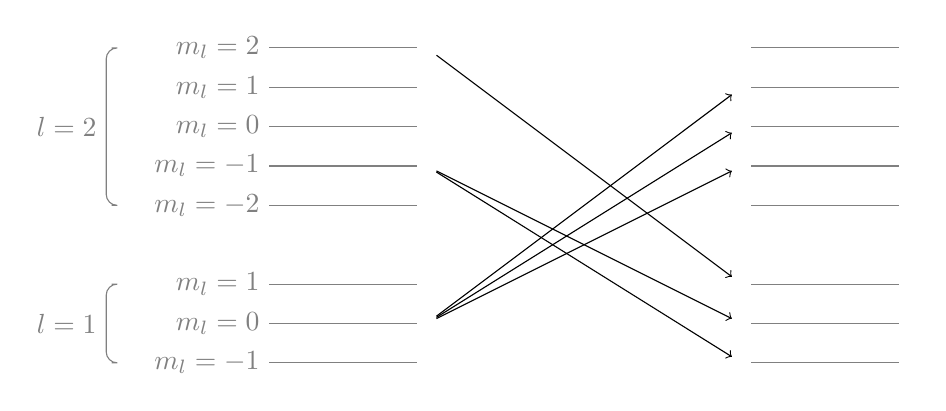
\begin{tikzpicture}
		% Sinistra
		\node (l1-1) at (-2,-1.5){};
		\node (l10)  at (-2,-1)  {};
		\node (l11)  at (-2,-0.5){};
		\node (l2-2) at (-2,0.5) {};
		\node (l2-1) at (-2,1)   {};
		\node (l20)  at (-2,1.5) {};
		\node (l21)  at (-2,2)   {};
		\node (l22)  at (-2,2.5) {};
		% Destra
		\node (r1-1) at (2,-1.5){};
		\node (r10)  at (2,-1)  {};
		\node (r11)  at (2,-0.5){};
		\node (r2-2) at (2,0.5) {};
		\node (r2-1) at (2,1)   {};
		\node (r20)  at (2,1.5) {};
		\node (r21)  at (2,2)   {};
		\node (r22)  at (2,2.5) {};
		% Raggruppamento delle linee con stesso n. quantico l
		\draw[rounded corners,black!50!white] (l1-1) ++(-4,0) -- ++(-2pt,0) to node[left]{$l=1$} ++(0,1) -- ++(2pt,0);
		\draw[rounded corners,black!50!white] (l2-2) ++(-4,0) -- ++(-2pt,0) to node[left]{$l=2$} ++(0,2) -- ++(2pt,0);
		% Linee spettrali non perturbate
		\draw[black!50!white] (l1-1) to +(-2,0) node[left]{$m_l=-1$};
		\draw[black!50!white] (l10)  to +(-2,0) node[left]{$m_l=0$};
		\draw[black!50!white] (l11)  to +(-2,0) node[left]{$m_l=1$};
		\draw[black!50!white] (l2-2) to +(-2,0) node[left]{$m_l=-2$};
		\draw[black!50!white] (l2-1) to +(-2,0) node[left]{$m_l=-1$};
		\draw[black!50!white] (l20)  to +(-2,0) node[left]{$m_l=0$};
		\draw[black!50!white] (l21)  to +(-2,0) node[left]{$m_l=1$};
		\draw[black!50!white] (l22)  to +(-2,0) node[left]{$m_l=2$};
		% Linee spettrali perturbate
		\draw[black!50!white] (r1-1) to +(2,0) node[right]{};
		\draw[black!50!white] (r10)  to +(2,0) node[right]{};
		\draw[black!50!white] (r11)  to +(2,0) node[right]{};
		\draw[black!50!white] (r2-2) to +(2,0) node[right]{};
		\draw[black!50!white] (r2-1) to +(2,0) node[right]{};
		\draw[black!50!white] (r20)  to +(2,0) node[right]{};
		\draw[black!50!white] (r21)  to +(2,0) node[right]{};
		\draw[black!50!white] (r22)  to +(2,0) node[right]{};
		% Frecce per indicare le transizioni tra i livelli
		\draw[thin,black,->] (l22) -- (r11);

		\draw[thin,black,->] (l2-1) -- (r10);
		\draw[thin,black,->] (l2-1) -- (r1-1);

		\draw[thin,black,->] (l10) -- (r21);
		\draw[thin,black,->] (l10) -- (r20);
		\draw[thin,black,->] (l10) -- (r2-1);
	\end{tikzpicture}
	\caption{Esempio della divisione di alcune linee spettrali dovuta all'effetto Zeeman normale.}
	\label{fig:zeeman-normale}
\end{figure}

Le transizioni tra livelli di energia di $\op H^{(0)}$ sono, come visto nel capitolo precedente, permesse solo se $\Delta l=\pm 1$ e $\Delta m_l=0,\pm 1$, quindi la variazione di energia tra i livelli perturbati è
\begin{equation}
	\Delta H=\Delta E^{(0)}+\frac{e\hbar B}{2mc}\Delta m_l
\end{equation}
da cui si nota che dove prima si aveva un livello, ora in corrispondenza ne osserviamo tre.
In realtà le osservazioni sperimentali mostrano che questa descrizione è sbagliata: si sono misurate più di tre linee anche non equidistanti tra loro.
Si è scoperto infatti che l'elettrone, come le altre particelle elementari, possiede un altro tipo di momento angolare, detto \emph{momento angolare intrinseco} o \emph{spin}, di cui non si è tenuto conto in queste equazioni.

\chapter{Sistemi con più gradi di libertà}
Salvo brevi eccezioni, finora abbiamo trattato solamente dei sistemi ad un grado di libertà, tipicamente una particella in moto lungo una retta.
Passiamo ora a studiare sistemi con più gradi di libertà, che possono corrispondere ad un maggior numero di particelle, all'aggiunta di altre dimensioni spaziali, o entrambe.
In questo capitolo ci occuperemo di introdurre lo schema matematico in cui inquadrare questi problemi, in via generale, per poterlo poi applicare a problemi più complessi di quelli già visti, come le rotazioni e gli atomi.

\section{Prodotto diretto di spazi vettoriali}
Il problema principale è capire come costruire lo spazio degli stati di tali sistemi.
Sappiamo che con un grado di libertà possiamo associare ad ogni stato un raggio in uno spazio di Hilbert complesso, separabile e infinito dimensionale.
Quando il sistema possiede più di una dimensione spaziale, tali dimensioni sono indipendenti e apportano ciascuna un grado di libertà; per ciascuna di esse abbiamo, ad esempio, un operatore della posizione e uno dell'impulso, e sappiamo già dai commutatori fondamentali che posizione e impulso di coordinate differenti commutano.
Analogamente, componendo più particelle in un sistema ciascuna di esse ha associata la coppia di operatori posizione e impulso (ad esempio) e tutti quelli che ne derivano.
/bin/bash: :wq: command not found
\begin{equation}
	\hilbert=\hilbert_1\otimes\hilbert_2\otimes\cdots\otimes\hilbert_d.
\end{equation}

Per studiare la definizione e le proprietà di base ci restringiamo ora al prodotto di due spazi $\hilbert_1$ e $\hilbert_2$.
Dati gli stati (qualsiasi) $\ket{A}\in\hilbert_1$ e $\ket{B}\in\hilbert_2$, possiamo costruire il loro prodotto diretto $\ket{A}\otimes\ket{B}$ che rappresenta lo stato del sistema combinato $\hilbert=\hilbert_1\otimes\hilbert_2$ in cui il sottosistema $\hilbert_1$ è nello stato $\ket{A}$ e il sottosistema $\hilbert_2$ è nello stato $\ket{B}$.
Chiaramente il prodotto non è commutativo, perch\'e in generale non è detto nemmeno che esista uno stato $\ket{A}$ in $\hilbert_2$ in modo da poter scrivere $\ket{B}\otimes\ket{A}$.
Lo spazio vettoriale $\hilbert_1\otimes\hilbert_2$ è dotato in modo naturale delle operazioni di somma e di moltiplicazione per scalare (un numero complesso) esattamente come gli spazi di partenza: esso contiene le coppie $\ket{A}\otimes\ket{B}$ per \emph{ogni} stato $\ket{A}\in\hilbert_1$ e ogni stato $\ket{B}\in\hilbert_2$, e tutte le possibili combinazioni lineari di essi.
Il \textit{bra} associato al \textit{ket} $\ket{A}\otimes\ket{B}$ è semplicemente $\bra{A}\otimes\bra{B}$; con questo, il prodotto interno nello spazio prodotto è definito come
\begin{equation}
	(\bra{A}\otimes\bra{B})(\ket{C}\otimes\ket{D})=\braket{A}{C}\braket{B}{D}
\end{equation}
che, in termini di probabilità, mostra come gli ``eventi'' nei due sistemi siano indipendenti, poich\'e la probabilità dell'evento composto risulta essere il prodotto delle singole probabilità.
Spesso lo stato composto si scrive omettendo il simbolo $\otimes$, o anche in un unico \textit{ket}, come
\begin{equation}
	\ket{A}\otimes\ket{B}\hspace{2cm}\ket{A}\ket{B}\hspace{2cm}\ket{A,B}.
\end{equation}
Utilizzeremo per un po' la prima e la terza notazione insieme.

Anche se possiamo costruire uno stato composto dal prodotto di due stati, non è vero che ogni stato del sistema composto si possa scrivere in tale modo: in generale, uno stato $\ket{\psi}\in\hilbert=\hilbert_1\otimes\hilbert_2$ è una combinazione lineare di stati composti.
Date due basi di autostati (eventualmente anche continui) $\ket{i}$ e $\ket{j}$ per gli spazi, una base dello spazio prodotto è l'insieme $\{\ket{i}\otimes\ket{j}=\ket{i,j}\}$, quindi in generale
\begin{equation}
	\hilbert\ni\ket{\psi}=\sum_{i,j}c_{ij}\ket{i,j}=\sum_{i,j}c_{ij}\ket{i}\otimes\ket{j}
\end{equation}
dove come al solito $c_{ij}=\braket{i,j}{\psi}=(\bra{i}\otimes\bra{j})\ket{\psi}$.
Solo nel caso in cui $c_{ij}$ si può scrivere nella forma $a_ib_j$ allora si ha
\begin{equation}
	\ket{\psi}=\sum_{i,j}a_ib_j\ket{i,j}=\sum_{i,j}a_i\ket{i}\otimes b_j\ket{j}=\bigg(\sum_ia_i\ket{i}\bigg)\otimes\bigg(\sum_jb_j\ket{j}\bigg)
\end{equation}
cioè $\ket{\psi}$ si può scrivere come prodotto di due stati semplici, e si dice talvolta \emph{separabile}.
Quando non esiste una tale fattorizzazione, lo stato è detto \emph{entangled}.\footnote{
	Letteralmente \textit{ingrovigliato}, \textit{intrecciato}.
	Il termine inglese è di uso comune, e raramente si trova tradotto in italiano.
}

Gli operatori nello spazio composto in generale sono, anche qui, combinazioni lineari di prodotti diretti di operatori di ciascuno spazio: dati due operatori $\op\xi^{(1)}$ e $\op\eta^{(2)}$ rispettivamente su $\hilbert_1$ e su $\hilbert_2$, possiamo associare ad essi l'operatore $\op\xi^{(1)}\otimes\op\eta^{(2)}$ sullo spazio composto tale che
\begin{equation}
	(\op\xi^{(1)}\otimes\op\eta^{(2)})(\ket{A}\otimes\ket{B})=(\op\xi^{(1)}\ket{A})\otimes(\op\eta^{(2)}\ket{B}).
\end{equation}
Notare come ogni operatore agisce soltanto sullo stato del ``proprio'' spazio, indipendentemente dal resto.
Ogni operatore di ciascuno spazio, d'altronde, si estende ad un operatore sullo spazio composto in modo naturale: l'operatore $\op\xi^{(1)}$ può essere esteso all'operatore
\begin{equation}
	\op\xi^{(1\otimes 2)}=\op\xi^{(1)}\otimes 1^{(2)}
\end{equation}
dove $1^{(2)}$ è l'identità dello spazio $\hilbert_2$.
Analogamente gli operatori di $\hilbert_2$ si estendono ad operatori del tipo $1^{(1)}\otimes\op\eta^{(2)}$.
Spesso ometteremo gli indici nei pedici, dato che nella maggior parte dei casi $\op\xi^{(1)}$ e $\op\xi^{(1)}\otimes 1^{(2)}$ rappresentano la stessa osservabile, solo definita in spazi diversi.\footnote{
	In generale però l'osservabile $\op\xi$ potrebbe non essere definita nell'altro spazio.
}
L'identità dello spazio composto è ovviamente $1^{(1)}\otimes 1^{(2)}$.
Come già anticipato, le osservabili $\op\xi$ e $\op\eta$ in questo caso fanno riferimento a sistemi differenti, dunque sono \emph{sempre compatibili}.
Una semplice conseguenza di questo fatto è che se $\op\xi\ket{\xi}=\xi\ket{\xi}$ e $\op\eta\ket{\eta}=\eta\ket{\eta}$, dove $\ket{\xi}\in\hilbert_1$ e $\ket{\eta}\in\hilbert_2$, allora
\begin{equation}
	\op\xi\op\eta\ket{\xi,\eta}=(\op\xi\otimes 1)(1\otimes\op\eta)(\ket{\xi}\otimes\ket{\eta})=\xi\eta\ket{\xi,\eta}
\end{equation}
cioè l'autovalore dello stato composto è il prodotto degli autovalori.
Un altro esempio è
\begin{equation}
	(\op\xi+\op\eta)\ket{\xi,\eta}=(\op\xi\otimes 1+1\otimes\op\eta)(\ket{\xi}\otimes\ket{\eta})=(\xi+\eta)\ket{\xi,\eta}
\end{equation}
Cos\`i come per gli stati, in generale un operatore non è il prodotto diretto di due operatori, e $\op\xi+\op\eta$ ne è un esempio.
Gli elementi di matrice di un operatore $\op\xi$ sullo spazio composto, data una base $\ket{i,j}$, si definiscono nel modo solito come $\xi_{iji'j'}\defeq\bra{i,j}\op\xi\ket{i',j'}$ in modo che
\begin{equation}
	\op\xi=\sum_{i,j,i',j'}\xi_{iji'j'}\ket{i,j}\bra{i',j'}
\end{equation}
e se $\op\xi$ si fattorizza nel prodotto $\op\eta\op\zeta=(\op\eta\otimes 1)(1\otimes\op\zeta)$ allora
\begin{equation}
	\bra{i,j}\op\xi\ket{i',j'}=\bra{i,j}\op\eta\op\zeta\ket{i',j'}=\bra{i}\op\eta\ket{i'}\bra{j}\op\zeta\ket{j'}
\end{equation}
cioè l'elemento di matrice dell'operatore prodotto non è altro che il prodotto degli elementi di matrice dei due fattori, nelle basi di ciascun singolo spazio.

\section{Oscillatore armonico isotropo}
Come primo facile esempio di sistema con più gradi di libertà riprendiamo l'oscillatore armonico in più dimensioni già visto a pagina \pageref{sec:oscillatore-armonico-multidimensionale}.
Per semplicità consideriamo solo due gradi di libertà, dato che la generalizzazione ad un numero maggiore è molto semplice.
Un oscillatore armonico è dato dal potenziale
\begin{equation}
	V(x_1,x_2)=\frac12m(\omega_1x_1^2+\omega_2x_2^2)
\end{equation}
ed è \emph{isotropo} se tutte le frequenze di oscillazione coincidono, in questo caso $\omega_1=\omega_2=\omega$.
L'hamiltoniano del sistema è dunque
\begin{equation}
	\op H=\frac1{2m}(p_1^2+p_2^2)+\frac12m\omega^2(x_1^2+x_2^2).
\end{equation}
Indichiamo i due gradi di libertà con dei generici indici 1 e 2 in quanto non sono necessariamente la due coordinate cartesiane di una particella in un piano, ma possono avere altri significati: i risultati che troveremo si applicano, senza alcun cambiamento, anche ad un sistema di due particelle in moto unidimensionale.
Con la notazione dei prodotti tensoriali che abbiamo introdotto, è chiaro che $\op x_1$ corrisponde all'operatore $\op x\otimes 1$ nello spazio composto, e analogamente $\op x_2=1\otimes\op x$, $\op p_1=\op p\otimes 1$ e $\op p_2=1\otimes\op p$.\footnote{
	Nell'indicare gli operatori composti omettiamo l'indice che indica a quale spazio si riferiscono, dato che è la stessa osservabile in spazi diversi.
	Lo spazio a cui fanno riferimento risulta comunque è ovvio in base alla posizione dell'operatore nel prodotto: $\op p\otimes 1$ è l'impulso del primo spazio, e cos\`i via.
}
Risulta inoltre che $(\op x\otimes 1)^2=\op x^2\otimes 1$ e analogamente per gli altri.
Allora l'hamiltoniano si riscrive come
\begin{equation}
	\begin{split}
		\op H&=\frac1{2m}(\op p^2\otimes 1+1\otimes\op p^2)+\frac12m\omega^2(\op x^2\otimes 1+1\otimes\op x^2)=\\
		&=\frac1{2m}(\op p^2\otimes 1+m^2\omega^2\op x^2\otimes 1+1\otimes\op p^2+m^2\omega^2 1\otimes\op x^2)=\\
		&=\frac1{2m}(\op p^2+m^2\omega^2\op x^2)\otimes 1+\frac1{2m}1\otimes(\op p^2+m^2\omega^2\op x^2)=\\
		&=\op H^{(1)}\otimes 1+1\otimes\op H^{(2)}
	\end{split}
\end{equation}
cioè l'hamiltoniano composto non è altro che la somma dei due hamiltoniani dei sottosistemi.
Dato che i due sistemi sono indipendenti, non interagiscono, ed è lecito aspettarsi che i due hamiltoniani rimangano ``separati''.
Se dunque $\ket{E_1}$ e $\ket{E_2}$ sono autostati, in ordine, dei due hamiltoniani con autovalori $E_1$ ed $E_2$, allora
\begin{multline}
	\op H(\ket{E_1}\otimes\ket{E_2})=
	(\op H^{(1)}\otimes 1)(\ket{E_1}\otimes\ket{E_2})+(1\otimes\op H^{(2)})(\ket{E_1}\otimes\ket{E_2})=\\=
	\op H^{(1)}\ket{E_1}\otimes\ket{E_2}+\ket{E_1}\otimes\op H^{(2)}\ket{E_2}=E_1\ket{E_1}\otimes\ket{E_2}+\ket{E_1}\otimes E_2\ket{E_2}=(E_1+E_2)\ket{E_1}\otimes\ket{E_2}
\end{multline}
cioè $\ket{E_1}\otimes\ket{E_2}$ è un autostato dell'hamiltoniano nel sistema composto.
Conosciamo già gli autostati dei singoli sistemi, ossia gli stati $\ket{n}$ tali che $\op H\ket{n}=(n+\frac12)\hbar\omega\ket{n}$: allora prese le basi $\{\ket{n_1}\}_{n_1=0}^{+\infty}$ e $\{\ket{n_2}\}_{n_2=0}^{+\infty}$ possiamo costruire la base del sistema composto data dagli stati
\begin{equation}
	\ket{n_1}\otimes\ket{n_2}=\ket{n_1,n_2}
\end{equation}
che sono tutti autostati dell'hamiltoniano, con autovalore $(n_1+n_2+1)\hbar\omega$.

La funzione d'onda, nelle variabili $x_1,x_2$ della posizione, dello stato composto è data da 
\begin{equation}
	\braket{x_1,x_2}{n_1,n_2}=(\bra{x_1}\otimes\bra{x_2})(\ket{n_1}\otimes\ket{n_2})=\braket{x_1}{n_1}\braket{x_2}{n_2}
\end{equation}
perciò la funzione d'onda dello stato composto è semplicemente il prodotto delle funzioni d'onda dei due sottosistemi: la notazione con il prodotto tensoriale rende subito evidente questo fatto.
\begin{figure}
	\tikzsetnextfilename{autofunzione-oscillatore2d-isotropo}
	\centering
	\begin{tikzpicture}
		\begin{axis}[
				xlabel=$x_1$,
				ylabel=$x_2$,
				view={-30}{50}
			]
			\addplot3[surf,domain=-3:3,domain y=-3:3,samples=50] function {(2*sqrt(pi))**(-1)*(2*x)**2*exp(-x**2)*(2**2*2!*sqrt(pi))**(-1)*(4*y**2-2)**2*exp(-y**2)}; % |1,2>
		\end{axis}
	\end{tikzpicture}
	\caption{Densità di probabilità $\abs{\psi(x_1,x_2)}^2$ dello stato $\ket{1}\otimes\ket{2}$ dell'oscillatore armonico isotropo in due dimensioni.}
	\label{fig:autofunzione-oscillatore2d-isotropo}
\end{figure}


\section{Buca di potenziale quadrata}
Consideriamo il sistema composto da una buca di potenziale quadrata e infinita, di lato $a$: è descritta dal potenziale
\begin{equation}
	V(x_1,x_2)=
	\begin{cases*}
		0		&se $0<x<a,\ 0<y<a$\\
		+\infty	&altrimenti
	\end{cases*}
\end{equation}
Possiamo interpretarla equivalentemente come una particella racchiusa in una buca bidimensionale o due particelle identiche nella medesima buca unidimensionale.
Sappiamo già che all'esterno della buca la funzione d'onda deve essere identicamente nulla, quindi consideriamo d'ora in poi solo l'interno.
L'hamiltoniano del sistema è
\begin{equation}
	\op H=\frac1{2m}(\op p_1^2+\op p_2^2)=\frac1{2m}(\op p^2\otimes 1+1\otimes\op p^2)
\end{equation}
che si scompone in modo ovvio in due hamiltoniani, uno per ciascun grado di libertà.
Gli autostati di $\op H$ del sistema composto saranno allora il prodotto tensoriale degli autostati dei singoli sistemi: poich\'e una buca di potenziale unidimensionale, con tale potenziale, ammette le autofunzioni
\begin{equation}
	\psi_n(x)=\sqrt{\frac2{a}}\sin\frac{n\pi x}{a}
	\hspace{1cm}\text{con }
	E_n=\frac{\hbar^2n^2\pi^2}{2ma^2}
\end{equation}
per l'autostato $\ket{n}$, il sistema composto ammetterà le autofunzioni
\begin{equation}
	\braket{x_1,x_2}{n_1,n_2}=\braket{x_1}{n_1}\braket{x_2}{n_2}=\frac2{a}\sin\frac{n_1\pi x_1}{a}\sin\frac{n_2\pi x_2}{a}
\end{equation}
con l'energia data dalla somma degli autovalori
\begin{equation}
	E=E_{n_1}+E_{n_2}=\frac{\hbar^2(n_1^2+n_2^2)\pi^2}{2ma^2}.
\end{equation}

\section{Particelle identiche}
Nella meccanica classica il moto di una particella è dato in maniera deterministica: una volta specificati posizione e momento in un certo istante, le equazioni del moto forniscono una soluzione (la traiettoria della particella) ben definita, ad ogni istante.
Quando abbiamo a che fare con sistemi di particelle identiche, quindi, possiamo immaginare di individuare in un istante di tempo ciascuna particella, e misurandone posizione e momento potremo seguirle per tutta la durata del moto, effettivamente distinguendole l'una dall'altra.
In meccanica quantistica, a causa del principio di indeterminazione, ciò non è più possibile: nemmeno il concetto di traiettoria non è più definito, in quanto se misuriamo con assoluta precisione la posizione di una particella allora il suo momento avrà un'incertezza infinita, e non abbiamo alcun modo di determinare all'istante successivo dove si troverà.
Non possiamo più quindi aggrapparci alle equazioni del moto per distinguere le particelle l'una dall'altra, e infatti se esse condividono lo stesso insieme di proprietà fisiche (spin, massa, etc.) esse diventano a tutti gli effetti \emph{indistinguibili}.
Anche gli stati fisici nello spazio di Hilbert dovranno quindi riflettere questo fatto, ossia preso uno stato di un certo numero di particelle, se scambiamo tra loro alcune particelle lo stato non deve cambiare (a meno del solito fattore di fase).

In termini più rigorosi, quando abbiamo un insieme di $n$ particelle e ne scambiamo alcune tra loro, effettuiamo una permutazione di $n$ elementi, che è un elemento del \emph{gruppo simmetrico} $S_n$.
Come conseguenza, gli stati nello spazio di Hilbert si trasformeranno secondo una rappresentazione di tale gruppo.
Quando le particelle sono indistinguibili (e lo supporremo sempre nel resto della sezione) l'hamiltoniano del sistema non può dipendere dalla ``numerazione delle particelle'', quindi sarà invariante rispetto a ciascuna permutazione $\Pi\in S_n$: in altre parole l'operatore $\op U(\Pi)$ che implementa la permutazione nello spazio di Hilbert commuta con l'hamiltoniano:
\begin{equation}
    [\op U(\Pi),\op H]=0.
    \label{eq:commutatore-permutazione-hamiltoniano}
\end{equation}
Sappiamo inoltre che tale permutazione lascia lo stato fisico invariato a meno di un fattore di fase, perciò $\op U(\Pi)$ realizza una rappresentazione unidimensionale di $S_n$: per qualsiasi $n\ge 2$ è noto che le uniche rappresentazioni unidimensionali di $S_n$ sono quella banale e la rappresentazione ``segno'', che assegna a ciascuna permutazione --- appunto --- il suo segno (anche detto parità).
Chiaramente la rappresentazione banale non è di alcun interesse, di conseguenza abbiamo
\begin{equation}
    \op U(\Pi)=\pm 1.
\end{equation}
La \eqref{eq:commutatore-permutazione-hamiltoniano} implica tra l'altro che $\op H$ e $\op U(\Pi)$ hanno una base di autostati in comune; preso uno di questi autostati, avremo
\begin{equation}
    \op U(\Pi)\ket{E}=\pm\ket{E}
\end{equation}
e per le equazioni del moto di Heisenberg tale autovalore $\pm 1$ rimane tale per tutti gli istanti di tempo, cioè $\Pi$ è una costante del moto: l'evoluzione temporale degli stati non può portare stati con autovalore $-1$ in stati con autovalore $1$, e viceversa.
Questo comportamento degli stati sotto l'azione delle permutazioni delle particelle divide dunque lo spazio di Hilbert in due sottospazi ortogonali: se $\hilbert$ è lo spazio degli stati di una particella singola, allora lo spazio $\hilbert^n=\hilbert\otimes\cdots\otimes\hilbert$ composto dal prodotto di $n$ copie identiche di $\hilbert$ si suddivide in
\begin{equation}
    \hilbert^n=\hilbert_{(S)}\oplus\hilbert_{(A)}
\end{equation}
dove $(S)$ indica gli stati \emph{simmetrici}, con autovalore $1$, che non cambiano segno in seguito alla permutazione, e $(A)$ indica gli stati \emph{antisimmetrici}, che hanno autovalore $-1$ e invece cambiano segno.
La proprietà di un sistema di particelle di possedere stati simmetrici o antisimmetrici dipende dalla natura delle particelle:
\begin{itemize}
    \item le particelle con stati simmetrici sono dette \emph{bosoni}, poich\'e seguono la statistica di Bose-Einstein;
    \item le particelle con stati antisimmetrici sono dette \emph{fermioni}, poich\'e seguono invece la statistica di Fermi-Dirac.
\end{itemize}
La statistica a cui obbediscono in realtà dipende soltanto dallo spin delle particelle: le particelle con spin semi-intero sono fermioni, mentre quelle con spin intero sono bosoni.\footnote{
    Ciascuna particella elementare ha un proprio spin caratteristico: ad esempio elettroni, neutrini e in generale tutti i quark e i leptoni hanno spin semi-intero e sono dunque fermioni, mentre le particelle mediatrici delle forze come i fotoni hanno spin intero.
}
Per le particelle composte, la statistica è determinata da quella delle particelle che le compongono: se una particella è composta (oltre al resto) da $k$ fermioni, scambiare due tali particelle composte equivale a scambiare $k$ coppie di fermioni, e questo determina il segno dello stato finale; lo scambio dei bosoni non ha invece alcun effetto.


\backmatter

% Bibliografia
\cleardoublepage
\phantomsection
\addcontentsline{toc}{part}{\bibname}
\nocite{*}
\printbibliography
=======
>>>>>>> Introdotto il prodotto diretto di spazi di Hilbert

% Indice
\cleardoublepage
\pdfbookmark[-1]{Indice}{contents}
\tableofcontents
\end{document}
